\documentclass{article}
\usepackage[utf8]{inputenc}
\usepackage{amsmath}
\usepackage{xcolor}
\usepackage[top=2cm, bottom=2cm, left=2cm, right=2cm]{geometry}
\setlength\parindent{0pt}

\usepackage{listings}
%\usepackage{color}
\usepackage{graphicx}
\usepackage{float}
\usepackage{caption}

\usepackage{verbatim}
\let\oldv\verbatim
\let\oldendv\endverbatim

%\userpackage{minted}

\definecolor{dkgreen}{rgb}{0,0.6,0}
\definecolor{gray}{rgb}{0.5,0.5,0.5}
\definecolor{mauve}{rgb}{0.58,0,0.82}
\definecolor{light-gray}{gray}{0.95}


\lstset{frame=tb,
  language=Java,
  aboveskip=6mm,
  belowskip=6mm,
  showstringspaces=false,
  columns=flexible,
  basicstyle={\small\ttfamily},
  numbers=none,
  numberstyle=\tiny\color{gray},
  keywordstyle=\color{blue},
  commentstyle=\color{dkgreen},
  stringstyle=\color{mauve},
  breaklines=true,
  breakatwhitespace=true,
  tabsize=3,
  backgroundcolor=\color{light-gray},
  language=Matlab
}

%\usepackage{natbib} replaced by line below to make refernces work
\usepackage[square,sort,comma,numbers]{natbib}
\usepackage[nottoc,numbib]{tocbibind} %to get references in table of contants
\usepackage{graphicx}

\usepackage{bm}

\usepackage{hyperref}
\hypersetup{
	colorlinks,
	citecolor=black,
	filecolor=black,
	linkcolor=black,
	urlcolor=black
}

\usepackage{mdframed}
\usepackage{lipsum} % for creating dummy text
\mdfdefinestyle{MyFrame}{%
	linecolor=black,	
	backgroundcolor=gray!20!white,
	skipbelow = 8mm,
	skipabove = 8mm}

\usepackage{scrextend}

\usepackage{multimedia}
\usepackage{media9}

\usepackage{booktabs}
\usepackage{adjustbox}

\title{Fys4150\\Project 5\\ }
\author{Peter Killingstad and Karl Jacobsen\\
\\
\url{https://github.com/kaaja/fys4150}}

\begin{document}
	
\maketitle

\section*{Note to instructurs reagarding Github repository}
If the above Github-link does not work, it is eighter because you have not yet accepted our invite to the repository, or you have not yet provided us with an e-mail addres available at Github so that we can invite you. The Github user you will be invited from is "kaaja". If the latter applies to you, please send us an e-mail with an e-mailadress available in Github or your Github username so that we can send you an invite. Our e-mailadresses: peter.killingstad@hotmail.com, karljaco@gmail.com.


\section*{Abstract}
Numerical finite difference schemes displaying the truncation error for the 1D (Forward Euler, Backward Euler and Crank-Nicolson) and the 2D (explicit and implicit) diffusion equation are derived and simulated. All schemes has truncation error that is 2nd order in space. Except Crank-Nicolson, which is 2nd order in time, all schemes are 1st order in time. Except for Forward Euler , all schmes are shown to be unconditionally stable. The Forward Euler scheme is found to be stable for $\Delta t/\Delta x^2 < 1/2$, in the 1D case, and stable for $\Delta t /h^2 < 1/4$ in the quadratic ($h = \Delta x = \Delta y$) 2D case. Analytical solutions for the 1D and the 2D diffusion equation are derived. All 1D schemes are implemented through the $\theta$-rule. Linear system formulations are derived for all schemes. In 1D a more efficient version of the original Thomas algorithm is derived. The general fixed point iteration scheme, wiht conditions for convergence and FLOP count, is presented and related to the implemented Jacobi algorithm and the implemented Gauss-Seidel algorithm. These iterative methods are showm to be very efficient compared to direct schemes like Gaussian elimination. Gauss-Seidel is shown to be more efficient than Jacbobi, Gauss-Seidel needing only $2/3$ of the iterations of Jacobi. Parallelization by use of Open MP is used and shown to give a speed up of 4. It is shown that numerical evaluation of the analytical solution is far more demanding than the evaluation of the numerical schemes. Gaussian quadrature is applied for integraions. The simulations confirm that Forward Euler is sensitive around the stability limit, both in the 1D and the 2d case. In 1D, Crank-Nicolson outperforms the other schemes.

\section{Introduction}
Partial differential equations (PDEs) describes most physical processes. Analytical solutions to PDEs are only known in a few special cases. Numerical solutions of PDEs are indespensable in modelling of physical processes. In this report we will derive the most used schemes for one of the most used PDEs, the diffusion equation. We will develop finite difference schemes for solution of the 1D and the 2D diffusion equation. For the 1D case we derive and implement the Forward Euler scheme, the Backward Euler scheme and the Crank-Nicolson scheme. For the 2D case we derive and implement an explicit scheme and an implicit scheme.\\

Numerical schemes involves approximations, and this implies errors. Knowledge about a numerical methods error is of great importance. All schemes we derive, will be derived from Taylor expansions, implying that we get terms representing the order of the truncation errors (the errors that is made by leaving out terms in the Taylor series). \\

Numerical instability is another type of error that may occour due to approximations. A numerical scheme can give unphysical results, being unstable by e.g. producing unphysical oscillations. We perform Neuman stability analysis on all the derived schemes, identifying which schemes that are conditionally stable and what the stability requirements are.\\

Calculation of errors can be done in many ways. A very good method to calculate errors, is to compare the numerical solutions to analytical solutions. In our special case, we are so lucky that there exists known analytical solutions. Knowledge about how to derive these analytical solutions in itself is important. We derive, in full detail, the analytical solutions for both the 1D and 2D case.\\

The word "error" always comes up when discussing numerical schemes, and it is very often mentioned along with another word: "efficiency". A scheme can produce as small an error as possible, but it is worth little if it cannot produce the results in a reasonable amount of time. Hence methods improving the efficiency of the schemes are very central when dealing with numerical simulations. Our schemes can be, and ars, written as linear systems. Typicall for PDEs, these systems involve large and sparse matrices. Standard methods like Gaussian elimination for solving linear system becomes very time consuming. Alternatives are needed. \\

We improve the efficiency of the 1D schemes by utilizing that the schemes, when written as the general $\theta$-scheme, are tridiagonal linear systems. The Thomas algorithm, which is much more efficient than e.g. Gaussian elimination and LU-decomposition, can be used for these systems. We further improve the efficiency of the Thomas algorithm by taking into account that all coefficients in the coefficient matrix of the linear system are constant.\\

For the 2D implicit scheme, the matrix is no longer tridiagonal, so the Thomas algorithm cannot be used anymore. Other efficient alternatives to direct methods like Gaussian elimination and LU-decomposition are necessary. Iterative methods is one answer. We set up a general iterative method, the fixed point iteration method, and present convergence conditions and FLOP counts for this method. It is seen that this method quickly has the potential of being much more efficient than e.g. Gaussian elimination. Further the Jacobi iteration method and the Gauss-Seidel iteration methodn are related to the fixed point iteration method, and then implemented to the implicit 2D scheme.\\

Improving the efficiency further, we parallize parts of our code, using open MP. A timing analysis reveals that evaluation of the analytical solution takes up considerably more time than the numerical schemes! As a result, we parallize the analytical solution. We also parallelize that Jacobi solver. \\

One reason for the high computational demands from evaluation of the analytical solution, is that there is a double integral that needs to be evaluated many times. In order to speed up the evaluation of this integral, we apply Gaussian quadrature with Legendre polynomials. Gaussian quadrature is known to be much more efficient compared to standard integration rules like e.g. Simpson's rule.\\

In the next section the analytical solution is derived, before we turn to derivation and error analysis of the numerical schemes. Finally results and conlcusions follows.

\section{Theory}
This section contains derivations of analytical solutions and derivation and error analysis of the numerical schemes. But first, the physical problems are presented.

\subsection{1D problem}
The one-dimensional problem is written as 

\begin{subequations}
	\begin{eqnarray}
	\frac{\partial^2 u(x,t)}{\partial x^2} &=& \frac{\partial u(x,t)}{\partial t} \textit{, } t> 0 \textit{, } x \in (0,L) \\ \nonumber
	\\
	u(x,0) &=& 0 \textit{, } 0 <x < 1 \textit{,} \\
	u(0,t) &=& 0 \textit{, } t>0 \\
	u(L,t) &=& 1 \textit{, } t>0,
	\end{eqnarray}
\end{subequations}

where the length has been scaled by the lenght of the $x$-domain, $L$.\\

The problem consists of non-homogeneous boundary conditions, and it is not trivial to find a closed form solution. The problem can be seen as a physical problem such as a temperature gradient in a rod or flow between two infinite flat plates, where the fluid is initially at rest and the plate at $x=1$ is given a sudden movement. 

\subsection{2D problem}
In the 2D case, we choose to model a laminar flow inside an infinite tunnel with a finite quadratic cross section. We only model a single cross section, the problem being identical for all cross sections because of the homogenity assumption in the flow direction. \\

There will be no slip boundary conditions on all four walls. The floor and the sides will be fixed, while the roof will be moving in the flow direction. With these boundary conditions we have zero velocity on the floor and the side walls, while we have a non-zero velcocity in the flow direction. The figure below shows our problem.

\begin{figure}[H]
	\centering
	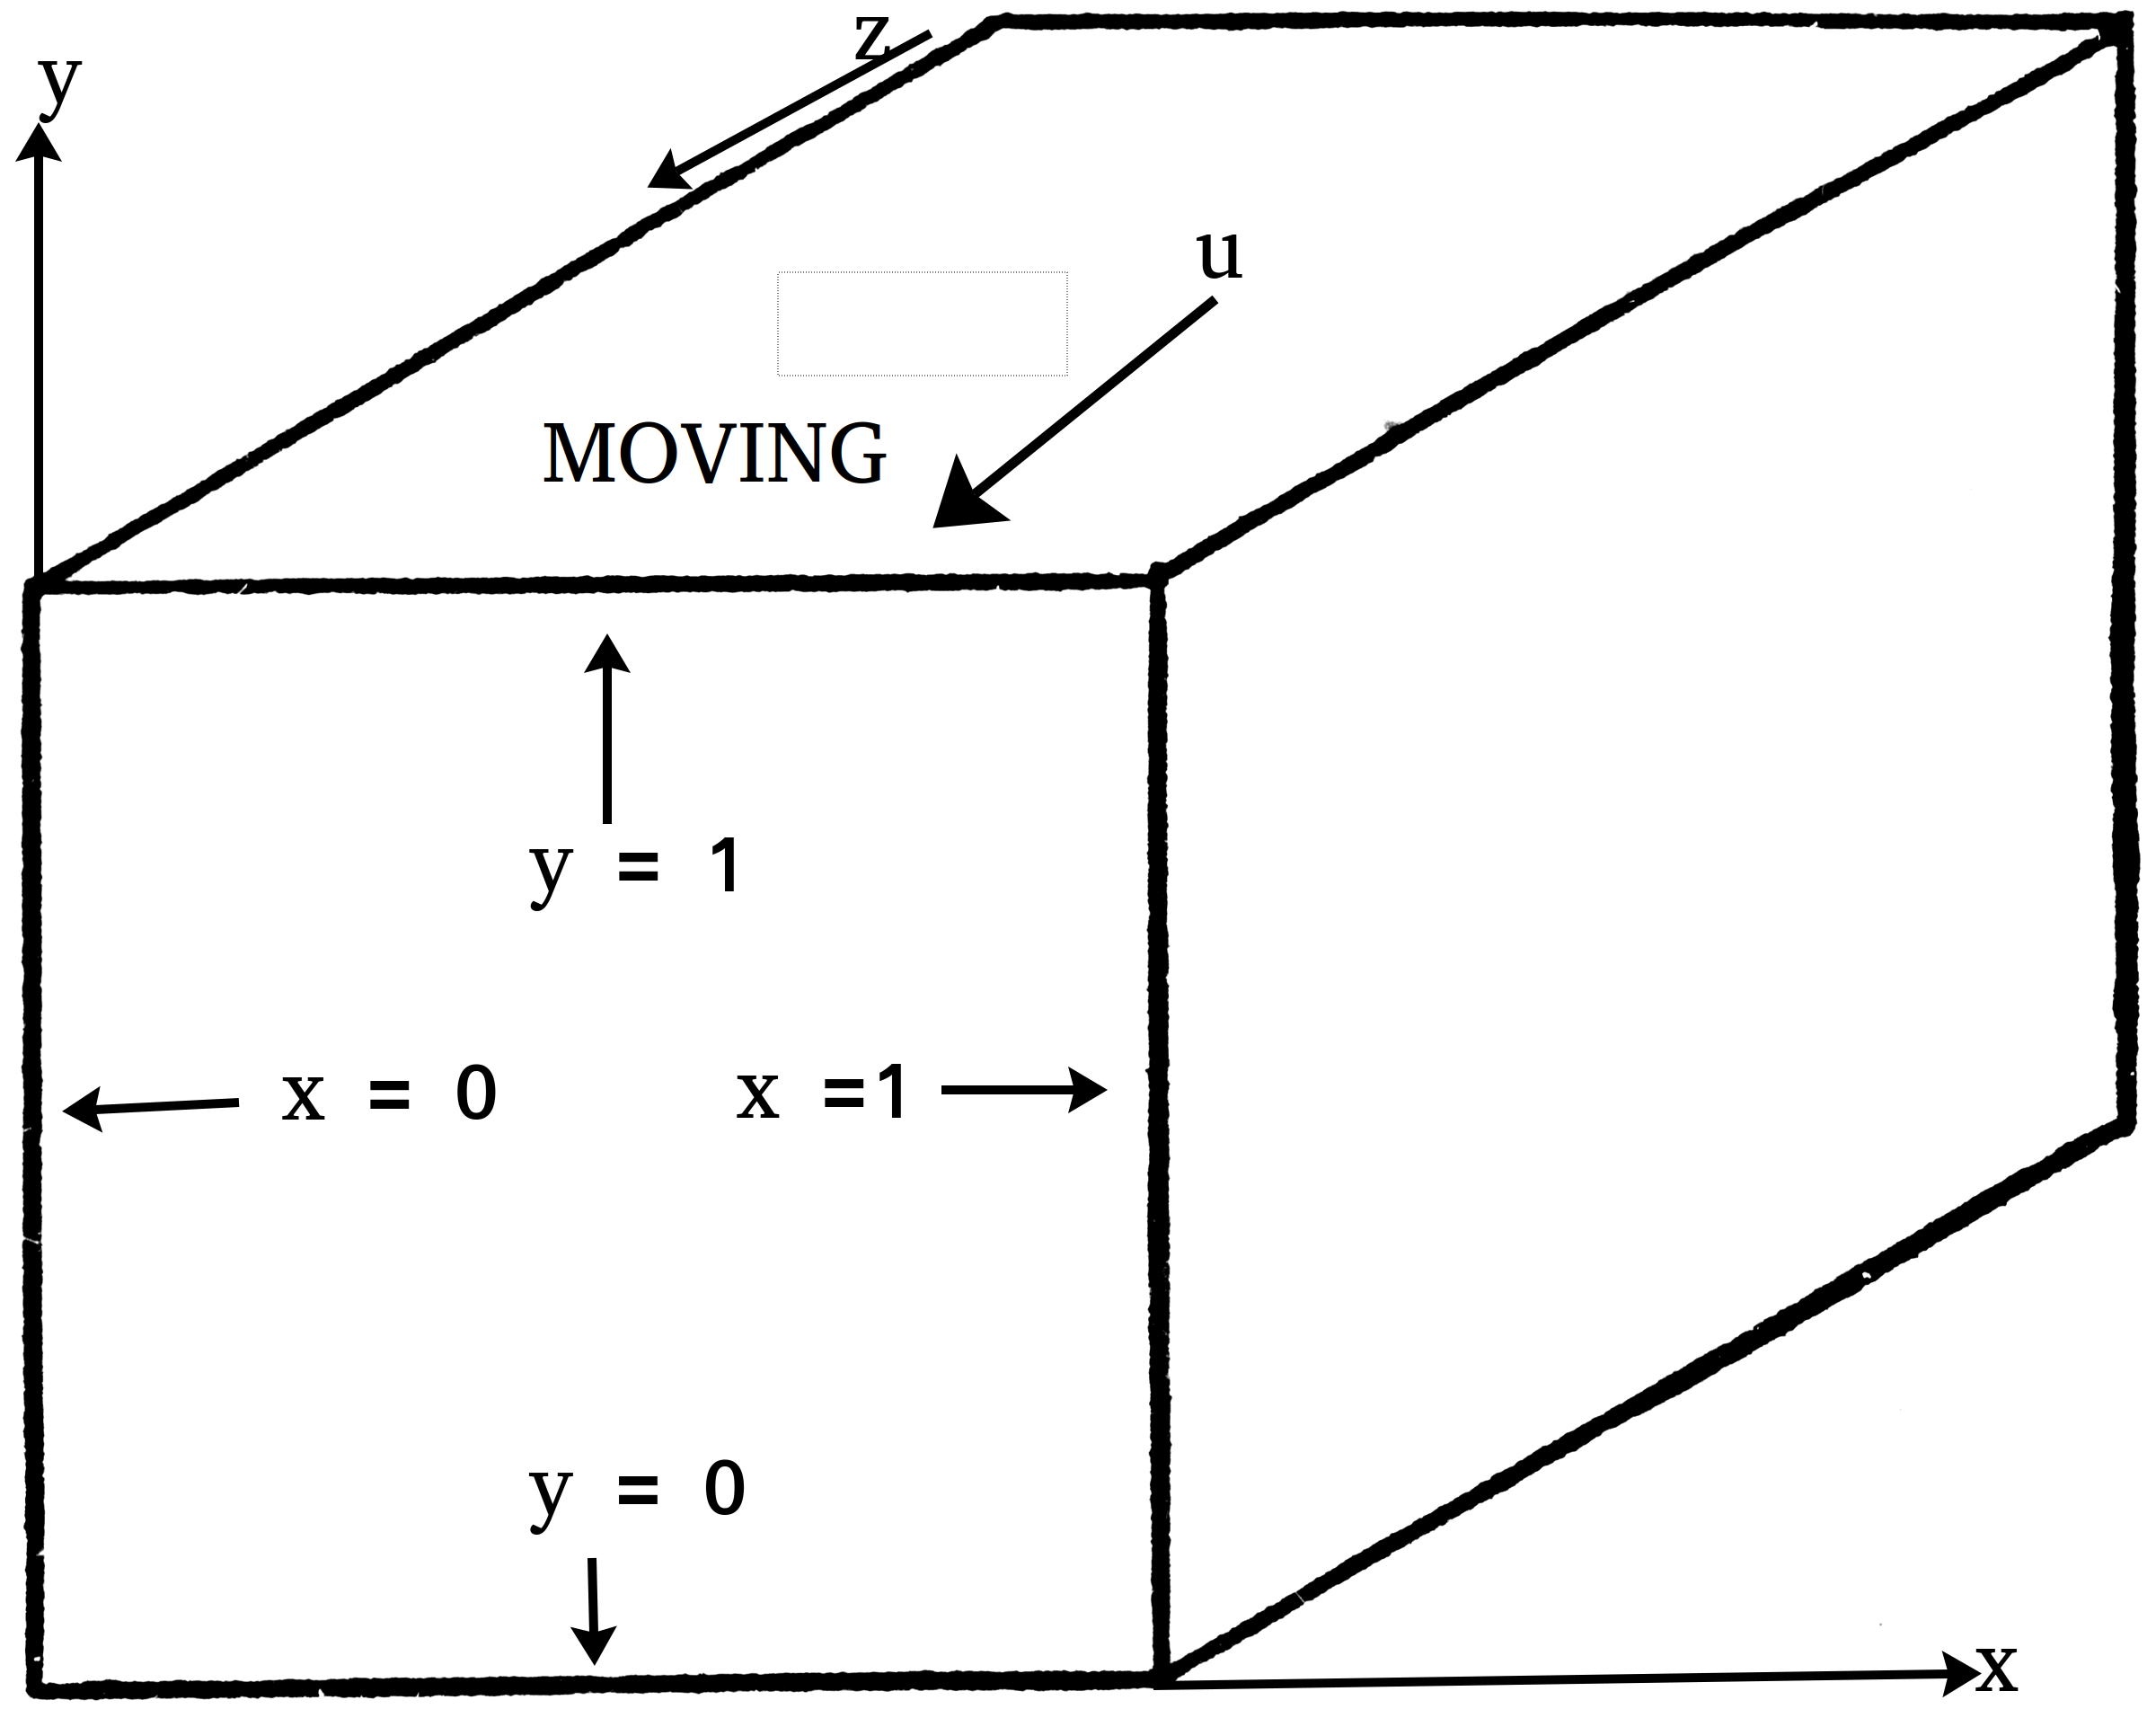
\includegraphics[width=0.6\textwidth]{/home/karl/doc/subj/att/fys4150/project5/resultsKeep/5e/boxDrawing2-0.png}
	\caption{2D problem sketch}
	\label{1}
\end{figure}

With our choise of coordinate system, positive flow represents flow out of the paper. \\

We choose $u(x,y=1) = 1$, and $u(x=0, y) = u(x=1,y) = u(x,y=0) = 0$. \\

We model the flow with the heat equation. This equation can be derived from the equations of incompressible flow, the Navier-Stokes equations, by assuming laminar flow and a flow profile of type $u = u(x,y)$:

\begin{subequations}
	\begin{align}
	\mathbf{u}_t + (\mathbf{u} \cdot \nabla) \mathbf{u} &= -\frac{\nabla p}{\rho} + \nabla^2 \mathbf{u}\\
	w(x,y)_t + (w \frac{\partial}{\partial z}) w(x,y) &\stackrel{\text{Zero pressure gradient}}{=} (\frac{\partial^2}{\partial x^2} + \frac{\partial^2}{\partial x^2} ) w(x,y)\\
	w(x,y)_t &= (\frac{\partial^2}{\partial x^2} + \frac{\partial^2}{\partial x^2} )w(x,y)\label{eq:ns}
	\end{align}
\end{subequations}

Central assumptions behind the resulting heat equation is that there is no external pressure gradient and that the flow is laminar. 

\subsection{Analytical solutions}

\subsubsection{Analytical solution 1D}


From physical observations we know that as time goes, i.e. when $t\rightarrow \infty$,  the problem coinsides whith its surroundings and becomes steady. It is reasonable to introduce a solution consisting of the sum of two parts, a steady-state solution, and a transient solution that depends on the initial conditions:

\begin{equation}
u(x,t) = U(x) + V(x,t)
\end{equation}
where $U(x)$ is the steady-state solution and $V(x,t)$ is the transient solution.\\ 

Since the steady-state problem is not changing in time, i.e. $\partial_ t = 0$, it is written in a compact form as:
\begin{subequations}
	\begin{eqnarray}
	\label{eqn:steadyStateSODE}
	U_{xx} &=& 0 \textit{ , } x \in (0,1)\\ \nonumber
	\\
	U(0) &=& 0 \textit{  } \\
	U(L) &=& 1
	\end{eqnarray}
\end{subequations}

For the transient part of the problem we have the problem written in compact form as:

\begin{subequations}
	\begin{eqnarray}
	\label{eqn:transientODE}
	V_t &=& V_{xx} \textit{ , } t>0 \textit{ , } x \in (0,1) \\ \nonumber
	\\
	\label{eqn:transientIC}
	V(x,0) &=& -U(x) \textit{ , } 0<x<1 \\
	V(0,t) &=& 0 \textit{ , } t>0 \\
	V(1,t) &=& 0 \textit{ , } t>0
	\end{eqnarray}
\end{subequations}


The steady state solution is solved by integrating (\ref{eqn:steadyStateSODE}) twice

\begin{eqnarray}
\nonumber
\int \frac{\partial^2 u(x,t)}{\partial x^2}\;dx &=& A \\ \nonumber
\int \frac{\partial u(x,t)}{\partial x}\;dx &=& \int Adx +B \\ \nonumber
\end{eqnarray}

and we end up with the general solution $U(x) = Ax + B$. Applying the boundary conditions at $x=0$ and $x=1$ we get that 

\begin{equation}
U(x) = x
\label{eqn:UsteadyState1D}
\end{equation}

The transient problem (\ref{eqn:transientODE}) has homogeneous boundary conditions, and we can solve it by seperation of variables. We start by making the anzats that $V(x,t) = T(t)X(x)$ so that we can rewrite (\ref{eqn:transientODE}) as:

\begin{equation}
XT'=X''T 
\end{equation}

Reordering the equation we get the following:

\begin{equation}
\frac{T'}{T} = \frac{X''}{X} = k,
\end{equation}
where $k$ is an unknown constant. The reason we can insert $k$ into the above equation, is that the sides depends on different varirables, and so equality between the sides is only acheived if both sides equals a constant. We have homogenuous BCs, and for this to be achieved when we solve the $X$-part of the above equaion, we must have $k <0$. As can be seen later, with $k\geq 0$ we would not be able to satisfy the homogenupus BCs. For computationaly ease, we set $k = -\lambda^2$, where $\lambda > 0$. \\

Starting with the $t$ dependent part, we get

\begin{eqnarray}
\frac{T'}{T} = -\lambda^2 \\ 
T' = -\lambda^2 T
\end{eqnarray}

The ODE can be solved by separation of variables

\begin{subequations}
	\begin{eqnarray}
	\label{eqn:solvingTdependentTransientTerm1D}
	\frac{1}{T}\frac{dT}{dt} = -\lambda^2 \\ 
	\Rightarrow \frac{1}{T} dT = -\lambda^2 dt\\
	\int \frac{1}{T}dT = - \int \lambda^2 dt \\
	\Rightarrow \ln(T) = -\lambda^2 + A
	\end{eqnarray}
\end{subequations}

The $t$ dependent term is then given by

\begin{equation}
T = Ae^{-\lambda^2 t}
\label{eqn:tdependentTransientTerm1D}
\end{equation}

We see that our assumption $\lambda > 0$ makes sense also for the $T$-solution, since we do not get blow-up as $t \rightarrow \infty$. \\

For the $x$ dependent term we get

\begin{subequations}
	\begin{eqnarray}
	X'' = -\lambda^2 X \\
	\Rightarrow X'' + \lambda^2 X = 0 
	\end{eqnarray}
\end{subequations}

We use an anzats $X=e^{\alpha x}$:

\begin{subequations}
	\begin{eqnarray}
	\alpha^2 e^{\alpha x} + \lambda^2 e^{\alpha x} &=& 0 \\ 
	\Rightarrow \alpha^2 &=& -\lambda^2 \\ 
	\Rightarrow \alpha &=& \pm \sqrt{-\lambda^2}
	\end{eqnarray}
\end{subequations}

Since we have $\lambda > 0$, we get our wanted trigonometric solution

\begin{equation}
X = Be^{-i\lambda x} + Ce^{i\lambda x},
\label{eqn:xDependenttransientTerm1D}
\end{equation}

which can be written as

\begin{equation}
X(x) = B\cos(\lambda x) + C\sin(\lambda x) 
\end{equation},

where the constants have changed.\\

Applying the boundary conditions we get that

\begin{eqnarray}
X(0) = B\cos(0) + C\sin(0) = 0 \\ 
X(1) = B\cos(\lambda) + C\sin(\lambda) = 0
\end{eqnarray}

From the first boundary condition wher $x=0$ we must have that $B=0$. We are lookong for non-trivial solutions of the problem, so for $x=1$ we must find the  values that gives $C\sin(\lambda)=0$. We know that\\ $\sin(n \pi) =0 \textit{ for } n = 1,2, \ldots $, which lets us determine that $\lambda = n \pi$.\\

Summing up, we have the following particular solutions for the transient part:

\begin{subequations}
	\begin{eqnarray}
	V_n(x,t) = A_ne^{-(n\pi)^2 t}\sin(n \pi x), n=1,2,...,\infty
	\end{eqnarray}
\end{subequations}

Since all particular solutions satisfy the PDE, and the BCs are homogenuous, all linear combinations of the particular solutions will also satisfy our problem, giving the general soultion of the transient problem

\begin{equation}
\sum_{n=1}^{\infty} a_ne^{-(n\pi)^2 t}\sin(n \pi x)
\label{eqn:FundamentalSolutionODE}
\end{equation}

The coefficients $a_n$ is found by applying the initial condidtion (IC)

\begin{equation}\label{eq:genSolTrans}
-U(x) = \sum_{n=1}^{\infty} a_n\sin(n \pi x) 
\end{equation}

To obtain an expression for the coefficients $a_n$ we use that the functions $\sin(n\pi x)$ is orthogonal to each other in the sense that 

\begin{equation}
\int_0^1 \sin(n\pi x) \sin(m\pi x) dx = 
\begin{cases} 0 & \quad \text{if } m \neq n\\
1/2 & \quad \text{if } m = n 
\end{cases}
\label{eqn:orhogonalSine}
\end{equation}

Using the above statement, multiplying \ref{eq:genSolTrans} by $\sin(m\pi x)$  and then integrating over $x$ over the domain, we get 

\begin{eqnarray}
\nonumber
- \int_0^1 U(x)\sin(m\pi x)\;dx &=& a_n \int_0^1 \sum_{n=1}^{\infty} \sin(m\pi x)\sin(n\pi x)\;dx = a_m\int_0^1 \sin^2(m\pi x)\;dx\\ \nonumber
&\Rightarrow& - \int_0^1 U(x)\sin(m\pi x) =\frac{a_m}{2}\\ 
&\Rightarrow& a_m = - 2\int_0^1 U(x)\sin(m\pi x) \;dx
\end{eqnarray}

Solving for $a_n$, applying the steady state solution (\ref{eqn:UsteadyState1D}), yields 

\begin{eqnarray}
\nonumber
a_n = -2 \int_0^1 x \sin(m\pi x) &=& \Big[\frac{2}{(m\pi)^2} \sin(m\pi x) + \frac{2x}{m\pi}\cos(m\pi x)\Big]_0^1 \\ 
\label{eqn:fourierCoefficients}
&\Rightarrow & a_n = \frac{2}{m\pi}(-1)^m
\end{eqnarray}
\newline

Putting the coefficient from (\ref{eqn:fourierCoefficients}) into the fundamental solutions (\ref{eqn:FundamentalSolutionODE}) we end up with the following solution for the transient problem:

\begin{equation}
V(x,t) = 2\sum_{n=1}^{\infty} \frac{(-1)^k}{n\pi} e^{-(n\pi)^2 t}\sin(n\pi x)
\label{eqn:transientSolution1D}
\end{equation}

Now we get an expression for the whole problem by putting combining the steady-state solution (\ref{eqn:UsteadyState1D}) and the transient solution (\ref{eqn:transientSolution1D}) such that we obtain 

\begin{equation}
u(x,t) = U(x) + V(x,t) = x + 2\sum_{n=1}^{\infty}e^{-(n\pi)^2 t} \frac{(-1)^k}{n\pi}
\sin(n\pi x)
\label{eqn:solution1D}
\end{equation}

\subsubsection{Analytical solution 2D}
In the two-dimensional case the differential equation becomes
\begin{subequations}
	\begin{eqnarray}
	\frac{\partial^2 u(x,y,t)}{\partial x^2} + \frac{\partial^2 u(x,y,t)}{\partial y^2} &=&  \frac{\partial u(x,y,t)}{\partial t} \textit{ , } t>0 \textit{ , } x,y \in (0,1) \\ \nonumber \\
	u(x,y,0) &=& 0 \textit{ , } x,y \in (0,1) \\ 
	u(0,y,t) &=& 0 \textit{ , } t> 0 \\
	u(1,y,t) &=& 0 \textit{ , } t> 0 \\
	u(x,0,t) &=& 0 \textit{ , } t> 0  \\
	u(x,1,t) &=& 1 \textit{ , } t> 0 
	\end{eqnarray}
\end{subequations}

The boundary conditions is extended in such a way that the physical problem can be that of a flow whitin a box with infinite plates in the streamwise direction ($z$), where the fluid is initially at rest and the plate at $y=1$ is given a sudden movement. We have "no slip" boundary conditions i.e. the fluid has zero movement on all boundaries except at $y=1$.\\

To obtain a closed form solution for the two-dimensional, we use the same argument as for the one-dimensional problem, i.e. we split the solution into a steady-state solution and a transient solution.\\

We end up with a solution defined as:
\begin{equation}
u(x,y,t) = U(x,y) + V(x,y,t)
\end{equation}
where $U(x,y)$ is the steady-state solution and $V(x,y,t)$ is the transient solution.\\

The steady-solution is then written in a compact form as:
\begin{subequations}
	\begin{eqnarray}
	U_{xx} + U_{yy} &=& 0 \textit{ , } x,y \in [0,1]\\ \nonumber
	\\
	U(0,y) &=& 0 \textit{  } \\
	U(1,y) &=& 0 \textit{  } \\
	U(x,0) &=& 0 \textit{  } \\
	U(x,1) &=& 1 \textit{  } 
	\end{eqnarray}
\end{subequations}

For the transient problem we have the propblem defined as:

\begin{subequations}
	\begin{eqnarray}
	\label{eqn:transientPDE}
	V_t &=& V_{xx} + V_{yy} \textit{ , } t>0 \textit{ , } x \in [0,1] \\ \nonumber
	\\
	\label{eqn:transientICPDE}
	V(x,0) &=& -U(x,y) \textit{ , } x,y \in [0,1] \\
	V(0,y,t) &=& 0 \textit{ , } t>0 \\
	V(1,y,t) &=& 0 \textit{ , } t>0 \\
	V(x,0,t) &=& 0 \textit{ , } t>0 \\
	V(x,1,t) &=& 0 \textit{ , } t>0 
	\end{eqnarray}
\end{subequations}

For the steady-state problem we have a 2D Laplacian equation, which we can solve by seperation of variables. We use the anzats that $U(x,y) = X(x)Y(y)$, so that we end up with:

\begin{eqnarray}
\nonumber
YX'' + XY''=0 \\ \nonumber
\frac{X''}{X} = - \frac{Y''}{Y} = -\beta^2
\end{eqnarray}

Due to the independence of the terms on each side of the equation, we can solve the equations separately, each equation becoming

\begin{equation}
\frac{X''}{X} = -\beta^2 \nonumber
\end{equation}

\begin{equation}
\frac{Y''}{Y} = \beta^2 \nonumber
\end{equation}

The sign on the right hand side in both of the above equations is determined by the fact that in the $x$ dependent term we have homogeneous boundaries, while in the $y$ dependent term we have non-homogeneous. By the same reasoning as in the 1D-case, homogenupus BCs in the $x$-direction, we get $\beta > 0$. \\

For the $x$ dependent term we get

\begin{eqnarray}
\nonumber
X'' = -\beta^2 X \\ \nonumber
\Rightarrow X'' + \beta^2 X = 0,
\end{eqnarray}

which has a similar solution as that of the transient $x$ dependent term in the one-dimensional case (\ref{eqn:xDependenttransientTerm1D}). With our choise of $\beta$, we get the wanted trigonometric form

\begin{equation}
X(x) = A\cos(\beta x) + B\sin(\beta x) \nonumber.
\end{equation}

Applying the boundary conditions, we end up with the term

\begin{equation}
X_n(x) = B_n\sin(n\pi x),
\label{eqn:xDependenSteadyState2D}
\end{equation}

were ${X_n(x)}$ is the family of particular solutions.\\

The $y$ dependent term can be rewritten as 

\begin{subequations}
	\begin{eqnarray}
	y'' = \beta^2 Y \\ 
	\Rightarrow Y'' - \beta^2 Y = 0 
	\end{eqnarray}
\end{subequations}

We are again using an anzats so that $Y = e^{\gamma y}$. This leaves us with the term

\begin{subequations}
	\begin{eqnarray}
	\gamma^2 e^{\gamma y} - \beta^2 e^{\gamma y} &=& 0 \\ 
	\Rightarrow \gamma^2 &=& \beta^2 \\ 
	\Rightarrow \gamma &=& \pm \beta,
	\end{eqnarray}
\end{subequations}

and we end up with the following expression

\begin{eqnarray}
Y_n(y) &=& C_ne^{-n\pi y} + D_ne^{n\pi y} \\ 
&\Rightarrow & C_n\cosh(n\pi y) + D_n\sinh(n\pi y)
\end{eqnarray}
for the family of particular solutions.
\\

The fundamental solutions of the steady-state is the given by
\begin{equation}
U(x,y) = \sum_{n=1}^{\infty} X(x)Y(y) = \sum_{n=1}^{\infty} B_n\sin(n\pi x)\Big(C_n\cosh(n\pi y) + D_n\sinh(n\pi y)\Big)
\end{equation}

Applying the the boundary of $U(x,0)$ to the equation above we get that $C_n$ must be zero. We are then left with the expression

\begin{equation}
U(x,y) = \sum_{n=1}^{\infty} c_n \sin(n\pi x)\sinh(n\pi y)
\label{eqn:UsteadyStatefundamentalSolutions}
\end{equation}

Applying the last boundary $U(x,1) = 1$ we must have that

\begin{equation}
1 = \sum_{n=1}^{\infty} c_n \sin(n\pi x)\sinh(n\pi)
\end{equation}

setting $d_n = c_n\sinh(n\pi)$ we get that 

\begin{equation}
1 = \sum_{n=1}^{\infty} d_n \sin(n\pi x)
\end{equation}

Using again that the functions $\sin(n\pi x)$ is orthogonal (\ref{eqn:orhogonalSine}), as in the 1D case, multiplying the above equation with $ \sin(m\pi x)$ and  then integrating over $x$ over the domain, we get that 

\begin{subequations}
	\begin{eqnarray}
	d_n = 2\int_0^1 \sin(m\pi x) dx = \frac{2}{m\pi}\Big(1-(-1)^m\Big)\\
	\Rightarrow c_n = \frac{2}{m\pi \sinh(m\pi)}\Big(1-(-1)^m\Big).
	\end{eqnarray}
\end{subequations}

Putting the coefficients $c_n$ back into the expression for the fundamental solutions (\ref{eqn:UsteadyStatefundamentalSolutions}), we end up with the following expression for the steady-state
\begin{subequations}
	\begin{eqnarray}
	U(x,y) &=& \frac{2}{\pi} \sum_{m=1}^{\infty} \frac{\sin(m\pi x)\sinh(m\pi y)}{\pi \sinh(m\pi)}\Big(1-(-1)^m \Big)\\ 
	&\Rightarrow & U(x,y) = \frac{4}{\pi} \sum_{m=1}^{\infty} \frac{\sin((2m-1)\pi x)\sinh((2m-1)\pi y)}{\pi \sinh((2m-1)\pi)}.
	\end{eqnarray}
\end{subequations}

For the transient problem we once again use the anzats that $V(x,y,t) = X(x)Y(y)T(t)$ in order to write the problem as

\begin{subequations}
	\begin{eqnarray}
	XYT' = YTX'' + XTY'' \\
	\Rightarrow \frac{T'}{T} = \frac{X''}{X} + \frac{Y''}{Y} = -k^2.
	\end{eqnarray}
\end{subequations}

Starting by solving the $t$ dependent term, which is solved in the same way as for the one-dimensional term (\ref{eqn:solvingTdependentTransientTerm1D}), we end up with the expression

\begin{equation}
T=Ae^{-k^2t}.
\label{eqn:2DtransientTdependentGeneralTerm}
\end{equation}

For the $x$ dependent part we have 

\begin{subequations}
	\begin{eqnarray}\label{eq:xOde}
	\frac{X''}{X} = -\frac{Y''}{Y} - k^2\\
	\Rightarrow \frac{X''}{X} = -\gamma^2,
	\end{eqnarray}
\end{subequations}

where 

\begin{equation}\label{eq:gamma}
	-\gamma^2 = \frac{Y^{''}}{Y} - k^2.
\end{equation}

(\ref{eq:xOde}) has the same solution form as the $x$ dependent transient one-dimensional term (\ref{eqn:xDependenttransientTerm1D}), as well as the steady state two-dimensional term (\ref{eqn:xDependenSteadyState2D}), so we end up with 

\begin{equation}
X(x) = B\cos(\gamma x) + C\sin(\gamma x)
\end{equation}

For the above equation to hold on the boundaries, we get  $B=0$ and $\gamma = n\pi, n=1,2,...,\infty$, so we end up with

\begin{equation}
X_n(x) = c_n\sin(n\pi x)
\label{eqn:2DtransientXdependentTerm}
\end{equation}

We are left with the $y$ dependent term, which is written as 

\begin{subequations}
	\begin{equation}
	\frac{Y''}{Y} = k^2 - \gamma^2\\
	\end{equation}
\end{subequations}

Solving for $Y$ we again use the anzats $Y=e^{\alpha y}$ and obtain the term

\begin{subequations}
	\begin{eqnarray}
	\alpha^2 e^{\alpha y} + (\gamma^2 - k^2)e^{\alpha y} = 0 \\
	\alpha^2 + \gamma^2 - k^2 = 0 \\
	\Rightarrow \alpha = \pm \sqrt{k^2 - \gamma^2} 
	\end{eqnarray}
\end{subequations}

We are looking for a solution on the form that satisfies the homogenupus BCs for the transient term, resulting in

\begin{equation}
Y = D\cos(\sqrt{k^2 - \gamma^2}y) + E\sin(\sqrt{k^2 - \gamma^2}y)
\end{equation}

For the above equation to satisfy the boundary conditions $Y(0) = 0$ and $Y(1) = 0$, we get that $D = 0$ and that $\sqrt{k^2 - \gamma^2} = m\pi,\; m = 1,2,...\infty$. The $Y$ term is then given by

\begin{equation}
Y_m(y) = E_m\sin(m\pi y)
\label{eqn:2DtransientYdependentTerm}
\end{equation}

We can now calculate the constant $k^2$,  $k^2 = \gamma^2 + (m\pi)^2 = (n\pi)^2 + (m\pi)^2$. Putting this back into the $t$ dependent transient term (\ref{eqn:2DtransientTdependentGeneralTerm}) we have that 

\begin{equation}
T = A_{nm}e^{-\pi^2(m^2+n^2)t}.
\label{eqn:2DtransientTdependentTerm}
\end{equation}

Combining the $x,y$ and $t$ dependent terms ((\ref{eqn:2DtransientXdependentTerm}), (\ref{eqn:2DtransientYdependentTerm}) and (\ref{eqn:2DtransientTdependentTerm}) respectively), we end up with the fundamental solution

\begin{equation}
V(x,y,t) = \sum_{n=1}^{\infty} \sum_{m=1}^{\infty} A_{mn}\sin(n\pi x)\sin(m\pi y)e^{-\pi^2(m^2+n^2)t}.
\end{equation}

To find the coefficients $A_{nm}$, we use the initial condition

\begin{equation}
-U(x,y) =  \sum_{n=1}^{\infty} \sum_{m=1}^{\infty} A_{mn}\sin(n\pi x)\sin(m\pi y)
\end{equation}

We can solve for the coefficient by again using the orthogonality from (\ref{eqn:orhogonalSine}), multiplying the equation above by $ \sin(p\pi x) \sin(q\pi y)$, and integrating over the $x$ and $y$ domain to get

\begin{subequations}
	\begin{eqnarray}
	\int_0^1 \int_0^1 -U(x,y) \sin(p\pi x)\sin(q\pi y) dxdy =  \frac{A_{pq}}{4}\\
	\Rightarrow A_{pq} = -4 \int_0^1 \int_0^1 U(x,y) \sin(p\pi x)\sin(qn\pi y)\; dxdy.
	\end{eqnarray}
\end{subequations}

Finally we can combine the steady-state solution and the transient solution in order to get the analytical expression

\begin{eqnarray}
u(x,y,t) &=& U(x,y) + V(x,y,t)\\ \nonumber
&=& U(x,y) + \sum_{n=1}^{\infty} \sum_{m=1}^{\infty} A_{mn}\sin(n\pi x)\sin(m\pi y)e^{-\pi^2(m^2+n^2)t},
\end{eqnarray}

where

\begin{equation}
U(x,y) = \frac{4}{\pi} \sum_{m=1}^{\infty} \frac{\sin((2m-1)\pi x)\sinh((2m-1)\pi y)}{\pi \sinh((2m-1)\pi)}
\end{equation}

and 

\begin{equation}
A_{mn} = -4 \int_0^1 \int_0^1 U(x,y) \sin(m\pi x)\sin(n\pi y) dxdy.
\end{equation}



\subsection{Numerical schemes}
All the schemes will be derived from Taylor series expansions, and the truncation error will be related to the remainder in the Taylor-series expansions. This remainder is the error we get when truncating the series by leaving out the remainder.\\

\subsubsection{Forward Euler}
For the time derivative, we expand $u(x, t + \Delta t)$ around $t$

\begin{subequations}
	\begin{align}
		u(x, t+ \Delta t)  = u(x,t) +  u_t(x,t) \Delta t + \mathcal{O}(\Delta t^2)\\
		\rightarrow u_t(x,t) = \frac{u(x, t+ \Delta t) - u(x,t)}{\Delta t} + \mathcal{O}(\Delta t)\label{eq:FeTime}
	\end{align}
\end{subequations}

The space derivative, which is a 2nd derivative, we derive by combining two Taylor series'

\begin{subequations}
	\begin{align}
		u(x + \Delta x,t) = u(x,t) + u_x(x,t)\Delta x + \frac{u_{xx}(x,t) \Delta x^2}{2} + \frac{u_{xxx}(x,t) \Delta x^3}{6} + \mathcal{O}(\Delta x^4)\label{eq:feSpace1}\\
		u(x - \Delta x,t) = u(x,t) - u_x(x,t)\Delta x + \frac{u_{xx}(x,t) \Delta x^2}{2} - \frac{u_{xxx}(x,t) \Delta x^3}{6} + \mathcal{O}(\Delta x^4)\label{eq:feSpace2}
	\end{align}
\end{subequations}

Now we add (\ref{eq:feSpace1}) and (\ref{eq:feSpace2}) and solve for $u_{xx}(x,t)$

\begin{subequations}
	\begin{align}
		\begin{split}
			\Big(u(x + \Delta x,t) + u(x - \Delta x,t) \Big) &= \Big(u(x,t) + u(x,t) \Big)\\ 
			&+ \Big(u_x(x,t)\Delta x + (- u_x(x,t)\Delta x) \Big)\\ 
			&+ \Big(\frac{u_{xx}(x,t) \Delta x^2}{2} +  \frac{u_{xx}(x,t) \Delta x^2}{2}\Big)\\ 
			&+ \Big(\frac{u_{xxx}(x,t) \Delta x^3}{6}  + (- \frac{u_{xxx}(x,t) \Delta x^3}{6}) \Big)\\ 
			&+ \Big(\mathcal{O}(\Delta x^4) + \mathcal{O}(\Delta x^4) \Big)
		\end{split}\\
		&= 2u(x,t) + u_{xx}(x,t) \Delta x^2 + \mathcal{O}(\Delta x^4)\\
		\rightarrow u_{xx}(x,t) &= \frac{u(x - \Delta x, t) - 2u(x,t) + u(x+ \Delta x, t)}{\Delta x^2} + \mathcal{O}(\Delta x^2)\label{eq:feSpace3}
	\end{align}
\end{subequations}

Combining (\ref{eq:FeTime}) and (\ref{eq:feSpace3}) we get the Forward Euler scheme

\begin{subequations}
	\begin{align}
		u_t(x,t) &= u_{xx}(x,t)\\
		\frac{u(x, t+ \Delta t) - u(x,t)}{\Delta t} + \mathcal{O}(\Delta t) &= 
		\frac{u(x - \Delta x, t) - 2u(x,t) + u(x+ \Delta x, t)}{\Delta x^2} + \mathcal{O}(\Delta x^2)\label{eq:fe}
	\end{align}
\end{subequations}

From (\ref{eq:fe}) we see that the scheme has a truncation error that goes like $\mathcal{O} (\Delta t)$ in time and $\mathcal{O}(\Delta x^2)$ in space.\\

We will analyze the stability of the Forward Euler scheme (\ref{eq:fe}) by applying Neuman stability analysis. From the analytical solution of the problem, we know that the particular solutions are on the form $u = e^{-(k \pi)^2 t}e^{i k \pi x}$, where $k$ is an integer greater than one. We observe that the solutions are stable in $t$, meaning that the solutions do not blow up as $t$ increaes. Based on the analytical particular solution, we make the numerical ansatz 

\begin{equation}\label{eq:neumanAnsatz}
	u = a_k^n e^{i k \pi x_j}
\end{equation}

For the numerical ansatz (\ref{eq:neumanAnsatz}) to reproduce the characteristics of the analytical particular solution, with stability in $t$, we observe that $|a_k^n| < 1$ is necessary. We now plug in the ansatz (\ref{eq:neumanAnsatz}) into the (\ref{eq:fe}) and derive an equation for $|a_k^n|$:

\begin{subequations}\label{eq:naumanFe0}
	\begin{align}
		\frac{u(x, t+ \Delta t) - u(x,t)}{\Delta t}  &= 
		\frac{u(x - \Delta x, t) - 2u(x,t) + u(x+ \Delta x, t)}{\Delta x^2} \\
		\frac{a_k^{n+1} e^{i k \pi (j+1) \Delta x} - a_k^n e^{i k \pi j \Delta x}}{\Delta t}  &= 
		\frac{a_k^{n} e^{i k \pi (j-1) \Delta x} - 2a_k^{n} e^{i k \pi j \Delta x} + a_k^{n} e^{i k \pi (j+1) \Delta x}}{\Delta x^2} \\
		a_k^{n} e^{i k \pi j \Delta x}\; \frac{a_k  -1}{\Delta t}  &= 
		a_k^{n} e^{i k \pi j \Delta x}\; \frac{ e^{-i k \pi \Delta x} - 2  +  e^{i k \pi  \Delta x}}{\Delta x^2} \\
		 \frac{a_k  -1}{\Delta t}  &= 
		 \frac{ e^{-i k \pi \Delta x} - 2  +  e^{i k \pi  \Delta x}}{\Delta x^2} \\
		 a_k &= 1 + \frac{\Delta t}{\Delta x^2} (e^{-i k \pi \Delta x} - 2  +  e^{i k \pi  \Delta x})\\
		 &= 1+ \frac{\Delta t}{\Delta x^2} \Big(2 \cos(k\pi\Delta x) - 2\Big)\\
		 &= 1+ 2\frac{\Delta t}{\Delta x^2} \Big( \cos(k\pi\Delta x) - 1\Big)\\
		 &= 1+ 2\frac{\Delta t}{\Delta x^2} \Big(- 2 \sin^2(\frac{k\pi\Delta x}{2}) \Big)\\
		 &=1 - 4\frac{\Delta t}{\Delta x^2} \sin^2(\frac{k\pi\Delta x}{2}) \\
		 |a_k| &= |1 - 4\frac{\Delta t}{\Delta x^2} \sin^2(\frac{k\pi\Delta x}{2})|\label{eq:neumanFe1}
	\end{align}
\end{subequations}

From (\ref{eq:neumanFe1}) we get
 
\begin{subequations}
	\begin{align}
		 &|a_k| < 1\; \text{if}\; ||1 - 4\frac{\Delta t}{\Delta x^2} \sin^2(\frac{k\pi\Delta x}{2})|| < 1 \\
		 &\rightarrow |1 - 4 \frac{\Delta t}{\Delta x^2}| < 1 \rightarrow |a_k| < 1\;\text{(Since $\sin^2(k \pi \Delta x/2)_{max}  = 1$)}\\
		 &\rightarrow 1 - 4 \frac{\Delta t}{\Delta x^2} > -1\\ 
		 &\rightarrow \frac{\Delta t}{\Delta x^2} < \frac{1}{2}\label{eq:neumanFe2}
	\end{align}
\end{subequations}

(\ref{eq:neumanFe2}) gives that the Forward Euler scheme is conditionally stable, and the condition that ensures stability.


\subsubsection{Backward Euler}
Here we will do the same as we did for Forward Euler above: Derive the scheme, including truncation errors, and analyze stability.\\

The only change compared to Forward Euler, is the time discretization, which now becomes

\begin{subequations}
	\begin{align}
	u(x, t- \Delta t)  = u(x,t) +  u_t(x,t) \Delta t - \mathcal{O}(\Delta t^2)\\
	\rightarrow u_t(x,t) = \frac{u(x, t) - u(x,t - \Delta t)}{\Delta t} + \mathcal{O}(\Delta t)\label{eq:beTime}
	\end{align}
\end{subequations}

The space discretization is the same as for Forward Euler, (\ref{eq:feSpace3}). Combining the space discretization (\ref{eq:feSpace3}) and (\ref{eq:beTime}) gives

\begin{subequations}
	\begin{align}
		\frac{u(x, t) - u(x,t - \Delta t)}{\Delta t} + \mathcal{O}(\Delta t) = \frac{u(x - \Delta x, t) - 2u(x,t) + u(x+ \Delta x, t)}{\Delta x^2} + \mathcal{O}(\Delta x^2)\label{eq:be1}
	\end{align}
\end{subequations}

We note that the truncation errors have the same asymptoptic behavior as for the Forward Euler scheme. \\

To analyze the stability of the Backward Euler scheme, we apply the same method as we did for Forward Euler and insert the ansatz (\ref{eq:neumanAnsatz}) into (\ref{eq:be1}) to get

\begin{subequations}
	\begin{align}
		\frac{u(x, t) - u(x,t - \Delta t)}{\Delta t}  &= \frac{u(x - \Delta x, t) - 2u(x,t) + u(x+ \Delta x, t)}{\Delta x^2} \\
		\frac{a_k^n e^{i k \pi j \Delta x} - a_k^{n-1} e^{i k \pi j \Delta x}}{\Delta t}  &= \frac{a_k^n e^{i k \pi (j -1)\Delta x} - 2a_k^n e^{i k \pi j \Delta x} + a_k^n e^{i k \pi (1 + j)\Delta x}}{\Delta x^2} \\
		a_k^n e^{i k \pi j \Delta x}\; \frac{1 - a_k^{-1}}{\Delta t}&=
		a_k^n e^{i k \pi j \Delta x}\; \frac{e^{-i k \pi \Delta x} - 2 + e^{i k \pi \Delta x}}{\Delta x^2}\\
		\frac{1 - a_k^{-1}}{\Delta t}&= \frac{e^{-i k \pi \Delta x} - 2 + e^{i k \pi \Delta x}}{\Delta x^2}\\
		a_k^{-1} &= 1 - \frac{\Delta t}{\Delta x^2} (e^{-i k \pi \Delta x} - 2 + e^{i k \pi \Delta x})\\
		a_k &= \frac{1}{1 - \frac{\Delta t}{\Delta x^2} (e^{-i k \pi \Delta x} - 2 + e^{i k \pi \Delta x})}\\
		&\stackrel{(\ref{eq:naumanFe0})}{=}  \frac{1}{1 + 4 \frac{\Delta t}{\Delta x^2} \sin^2(\frac{k\pi\Delta x}{2})}\\
		|a_k| &=  \left|\frac{1}{1 + 4 \frac{\Delta t}{\Delta x^2} \sin^2(\frac{k\pi\Delta x}{2})}\right| < 1.\label{eq:neumanBe}\\
	\end{align}
\end{subequations}

From (\ref{eq:neumanBe}) we see that, in contrast to the Forward Euler scheme, the Backward Euler scheme is unconditionally stable.\\

(\ref{eq:be1}) reveals another difference between the Backward Euler scheme and the Forward Euler scheme: (\ref{eq:be1}) is implicit in $u(x,t)$, meaning that we cannot solve (\ref{eq:be1}) directly for $u(x,t)$, as we did in the Forward Euler scheme. However, we can find $u(x,t)$ from (\ref{eq:be1}) by recognizing that (\ref{eq:be1}) can be rewritten as a linear system:

\begin{subequations}
	\begin{align}
		\frac{u(x, t) - u(x,t - \Delta t)}{\Delta t}  &= \frac{u(x - \Delta x, t) - 2u(x,t) + u(x+ \Delta x, t)}{\Delta x^2} \\
		\frac{u_i^n - u_i^{n-1}}{\Delta t}  &= \frac{u_{i-1}^n - 2u_i^n + u_{i+1}^n}{\Delta x^2} \\
		\frac{\Delta x^2}{\Delta t}(u_i^n - u_i^{n-1})  &=  u_{i-1}^n - 2u_i^n + u_{i+1}^n\\
		- \Big(u_{i-1}^n - (2 + \frac{\Delta x^2}{\Delta t}) u_i^n + u_{i+1}^n\Big)   &=  \frac{\Delta x^2}{\Delta t}u_i^{n-1}\\
		 \Big(-u_{i-1}^n + (2 + \frac{\Delta x^2}{\Delta t}) u_i^n - u_{i+1}^n\Big)   &=  \frac{\Delta x^2}{\Delta t}u_i^{n-1}\\
		\underbrace{\begin{bmatrix} 2 + \frac{\Delta x^2}{\Delta t} & -1 & \cdots & 0 \\ -1 & 2 + \frac{\Delta x^2}{\Delta t} & -1 & \vdots \\
			\vdots & &  \ddots & \vdots \\ 
			0 & \cdots & -1 & 2 + \frac{\Delta x^2}{\Delta t} \end{bmatrix}}_{\mathbf{A}} 
		\underbrace{\begin{bmatrix} u_1^n\\ u_2^n \\ \vdots\\ u_N^n \end{bmatrix}}_{\mathbf{U}} &= 
		\underbrace{\frac{\Delta x^2}{\Delta t} \begin{bmatrix} u_0^{n-1}\\ u_1^{n-1} \\ \vdots \\ u_N^{n-1}\end{bmatrix}}_{\mathbf{\tilde{b}}}\label{eq:beLinSys}
	\end{align}
\end{subequations}

We see from (\ref{eq:beLinSys}) that solving Backward Euler corresponds to solving a linear system $A U = \tilde{b}$, where $A$ is a trdiagonal matrix. 
	
\subsubsection{Crank-Nicolson}
Here we Taylor expand $u(x+\Delta x, t+\Delta t)$ and $u(x-\Delta x, t+\Delta t)$ around $t'=t+\Delta t/2$ to get

\begin{subequations}
	\begin{align}
		\begin{split}
			u(x+\Delta x, t+\Delta t)&=u(x,t')+\frac{\partial u(x,t')}{\partial x}\Delta x+\frac{\partial u(x,t')}{\partial t} \frac{\Delta t}{2} +\frac{\partial^2 u(x,t')}{2\partial x^2}\Delta x^2 +\frac{\partial^3 u(x,t')}{6\partial x^3}\Delta x^3\\
			&+\frac{\partial^2 u(x,t')}{2\partial t^2}\frac{\Delta t^2}{4} 
			+\frac{\partial^2 u(x,t')}{\partial x\partial t}\frac{\Delta t}{2} \Delta x+ \mathcal{O}(\Delta t^3) + \mathcal{O}(\Delta x^4)
		\end{split}\label{eq:cn1}\\
		\begin{split}
			u(x-\Delta x,t+ \Delta t)&=u(x,t')
			-\frac{\partial u(x,t')}{\partial x}\Delta x 
			+ \frac{\partial u(x,t')}{\partial t} \frac{\Delta t}{2} + 
			\frac{\partial^2 u(x,t')}{2\partial x^2}\Delta x^2 
			-\frac{\partial^3 u(x,t')}{6\partial x^3}\Delta x^3\\
			&+\frac{\partial^2 u(x,t')}{2\partial t^2}\frac{\Delta t^2}{4} 
			- \frac{\partial^2 u(x,t')}{\partial x\partial t}\frac{\Delta t}{2} \Delta x
			+ \mathcal{O}(\Delta t^3) + \mathcal{O}(\Delta x^4)
		\end{split}\label{eq:cn2}\\
		\begin{split}
			u(x+\Delta x,t)&=u(x,t')
			+\frac{\partial u(x,t')}{\partial x}\Delta x
			-\frac{\partial u(x,t')}{\partial t} \frac{\Delta t}{2} +\frac{\partial^2 u(x,t')}{2\partial x^2}\Delta x^2
			 +\frac{\partial^3 u(x,t')}{6\partial x^3}\Delta x^3\\
			&+\frac{\partial^2 u(x,t')}{2\partial t^2}\frac{\Delta t^2}{4} 
			- \frac{\partial^2 u(x,t')}{\partial x\partial t}\frac{\Delta t}{2} \Delta x+ \mathcal{O}(\Delta t^3) + \mathcal{O}(\Delta x^4)
		\end{split}\label{eq:cn3}\\
		\begin{split}
		u(x-\Delta x,t)&=u(x,t')-\frac{\partial u(x,t')}{\partial x}\Delta x-\frac{\partial u(x,t')}{\partial t} \frac{\Delta t}{2} 
		+ \frac{\partial^2 u(x,t')}{2\partial x^2}\Delta x^2
		-\frac{\partial^3 u(x,t')}{6\partial x^3}\Delta x^3\\
		&
		+\frac{\partial^2 u(x,t')}{2\partial t^2}\frac{\Delta t^2}{4}
		+\frac{\partial^2 u(x,t')}{\partial x\partial t}\frac{\Delta t}{2} \Delta x
		+ \mathcal{O}(\Delta t^3) + \mathcal{O}(\Delta x^4)
		\end{split}\label{eq:cn4}\\
		u(x,t+\Delta t)&=u(x,t')+\frac{\partial u(x,t')}{\partial t}\frac{\Delta_t}{2} +\frac{\partial ^2 u(x,t')}{2\partial t^2}\Delta t^2 + \mathcal{O}(\Delta t^3)\label{eq:cn5}\\
		u(x,t)&=u(x,t')-\frac{\partial u(x,t')}{\partial t}\frac{\Delta t}{2}+\frac{\partial ^2 u(x,t')}{2\partial t^2}\Delta t^2 + \mathcal{O}(\Delta t^3)\label{eq:cn6}
	\end{align}
\end{subequations}

The above formulae are taken from Hjorth-Jensen's  \href{https://github.com/CompPhysics/ComputationalPhysics/tree/master/doc/pub/pde}{slides} \cite{MHJ2}.\\

Combining (\ref{eq:cn5}) and (\ref{eq:cn6}) gives the time derivative

\begin{subequations}
	\begin{align}
		\begin{split}
			\Big(u(x,t+\Delta t) - u(x,t)\Big) &= \Big(u(x,t') -  u(x,t')\Big) + \Big(\frac{\partial u(x,t')}{\partial t}\frac{\Delta_t}{2} - (-\frac{\partial u(x,t')}{\partial t}\frac{\Delta t}{2}) \Big)\\ 
			&+ \Big(\frac{\partial ^2 u(x,t')}{2\partial t^2}\Delta t^2 - \frac{\partial ^2 u(x,t')}{2\partial t^2}\Delta t^2 \Big) +\Big(\mathcal{O}(\Delta t^3) -  \mathcal{O}(\Delta t^3)\Big)
		\end{split}\\
		u(x,t+\Delta t) - u(x,t)& = \frac{\partial u(x,t')}{\partial t}\Delta t + \mathcal{O}(\Delta t^3)\\
		\frac{\partial u(x,t')}{\partial t}&= \frac{u(x,t+\Delta t) - u(x,t)}{\Delta t} + \mathcal{O}(\Delta t^2)\label{eq:cnTime}
	\end{align}
\end{subequations}

Now for the spacial derivative. First we solve (\ref{eq:cn1}) and (\ref{eq:cn2}) for $u_{xx}(x, t')$

\begin{subequations}
	\begin{align}
		\begin{split}
		u(x+\Delta x, t+\Delta t) + u(x-\Delta x,t + \Delta t) &= 
		\Big(u(x,t') + u(x,t') \Big) + \Big(\frac{\partial u(x,t')}{\partial x}\Delta x-\frac{\partial u(x,t')}{\partial x}\Delta x\Big)\\ 
		&+ \Big(\frac{\partial u(x,t')}{\partial t} \frac{\Delta t}{2} +\frac{\partial u(x,t')}{\partial t} \frac{\Delta t}{2} \Big) + \Big(\frac{\partial^2 u(x,t')}{2\partial x^2}\Delta x^2+\frac{\partial^2 u(x,t')}{2\partial x^2}\Delta x^2\Big)\\
		&+ \Big(\frac{\partial u(x,t')}{\partial t} \frac{\Delta t}{2} +\frac{\partial u(x,t')}{\partial t} \frac{\Delta t}{2} \Big) + \Big(\frac{\partial^3 u(x,t')}{6\partial x^3}\Delta x^3-\frac{\partial^3 u(x,t')}{6\partial x^3}\Delta x^3\Big)\\
		& + \Big(\frac{\partial^2 u(x,t')}{2\partial t^2}\frac{\Delta t^2}{4} +\frac{\partial^2 u(x,t')}{2\partial t^2}\frac{\Delta t^2}{4} \Big) + \Big(\frac{\partial^2 u(x,t')}{\partial x\partial t}\frac{\Delta t}{2} \Delta x - \frac{\partial^2 u(x,t')}{\partial x\partial t}\frac{\Delta t}{2} \Delta x\Big)\\
		& + \Big(\mathcal{O}(\Delta t^3) + \mathcal{O}(\Delta t^3) \Big) + \mathcal{O}(\Delta x^4)
		\end{split}\\
		\begin{split}
			&=2u(x,t') + \frac{\partial u(x,t')}{\partial t} \Delta t
			+ \frac{\partial^2 u(x,t')}{\partial x^2}\Delta x^2
			 + \frac{\partial^2 u(x,t')}{2\partial t^2}\frac{\Delta t^2}{2}  
			 + \mathcal{O}(\Delta t^3) + \mathcal{O}(\Delta x^4)
		\end{split}\\
		\begin{split}
			&=2u(x,t') + \frac{\partial u(x,t')}{\partial t} \Delta t
			+ \frac{\partial^2 u(x,t')}{\partial x^2}\Delta x^2			
			+ \mathcal{O}(\Delta t^2) + \mathcal{O}(\Delta x^4)
		\end{split}\\	
		\begin{split}
		\frac{\partial^2 u(x,t')}{\partial x^2}\Delta x^2
		& = 
		u(x+\Delta x, t+\Delta t) + u(x-\Delta x,t + \Delta t) 
		- 2u(x,t') 
			\\ 
		&+\frac{\partial u(x,t')}{\partial t} \Delta t
		+  \mathcal{O}(\Delta t^2) + \mathcal{O}(\Delta x^4)
		\end{split}\\
		\begin{split}
			\frac{\partial^2 u(x,t')}{\partial x^2}
			&=\frac{u(x-\Delta x,t+ \Delta t)  - 2u(x,t') +  	u(x+\Delta x, t+\Delta t)}{\Delta x^2}\\
			& +\frac{\partial u(x,t')}{\partial t} \frac{\Delta t}{\Delta x^2} +\mathcal{O}(\Delta t^2) + \mathcal{O}(\Delta x^2)\label{eq:cnX2}
		\end{split}		
	\end{align}
\end{subequations}

Doing the same as in (\ref{eq:cnX2}) for (\ref{eq:cn3}) and (\ref{eq:cn4}) we obtain

\begin{subequations}\label{eq:cnX3}
	\begin{align}
		\begin{split}
			\frac{\partial^2 u(x,t')}{\partial x^2} &=\frac{u(x-\Delta x,t) - 2u(x,t') + u(x+\Delta x, t)}{\Delta x^2}\\
			&- \frac{\partial u(x,t')}{\partial t} \frac{\Delta t}{\Delta x^2} 
			+  \mathcal{O}(\Delta t^2) + \mathcal{O}(\Delta x^2)
		\end{split}
	\end{align}
\end{subequations}

Now we take the mean of (\ref{eq:cnX2}) and (\ref{eq:cnX3}) 

\begin{subequations}
	\begin{align}
		\begin{split}
			u_{xx}(x, t^{'}) &=\frac{1}{2} \Big(\frac{u(x-\Delta x,t+ \Delta t)  - 2u(x,t') +  	u(x+\Delta x, t+\Delta t)}{\Delta x^2} +\frac{\partial u(x,t')}{\partial t} \frac{\Delta t}{\Delta x^2} + \mathcal{O}(\Delta t^2) + \mathcal{O}(\Delta x^2) \\
			&+  \frac{u(x-\Delta x,t) - 2u(x,t') + u(x+\Delta x, t)}{\Delta x^2} -\frac{\partial u(x,t')}{\partial t} \frac{\Delta t}{\Delta x^2} + \mathcal{O}(\Delta t^2)  + \mathcal{O}(\Delta x^2)\Big)\\
			&= \frac{1}{2} \Big(\frac{u(x-\Delta x,t+ \Delta t)  - 2u(x,t') +  	u(x+\Delta x, t+\Delta t)}{\Delta x^2} \\
			& +  \frac{u(x-\Delta x,t) - 2u(x,t') + u(x+\Delta x, t)}{\Delta x^2} \Big) + \mathcal{O}(\Delta t^2) + \mathcal{O}(\Delta x^2)\\
			&\stackrel{u(x,t^{'}) = \frac{u(x,t) + u(x,t+\Delta t)}{2}}{=}
			\frac{1}{2} \Big(\frac{u(x-\Delta x,t+ \Delta t)  - u(x,t) + u(x,t+\Delta t) +  	u(x+\Delta x, t+\Delta t)}{\Delta x^2} \\
			& +  \frac{u(x-\Delta x,t) - u(x,t) + u(x,t+\Delta t) + u(x+\Delta x, t)}{\Delta x^2} \Big) + \mathcal{O}(\Delta t^2) + \mathcal{O}(\Delta x^2)\\
			&= \frac{1}{2} \Big(\frac{u(x-\Delta x,t+ \Delta t) - 2u(x,t+\Delta t) +u(x + \Delta x,t+\Delta t)}{\Delta x^2} + \frac{u(x-\Delta x,t) - 2u(x,t) +u(x+ \Delta x,t)}{\Delta x^2} \Big)\\
			& + \mathcal{O}(\Delta t^2)  + \mathcal{O}(\Delta x^2)\label{eq:cnX4}
			\end{split}
	\end{align}
\end{subequations}

Now combining (\ref{eq:cnTime}) and (\ref{eq:cnX4}) we get the Crank-Nicolson scheme

\begin{subequations}\label{eq:cn1d}
	\begin{align}
		\begin{split}
			\frac{u(x,t+\Delta t) - u(x,t)}{\Delta t} + \mathcal{O}(\Delta t^2)
			&= \frac{1}{2} \Big(\frac{u(x-\Delta x,t+ \Delta t)
			- 2u(x,t+\Delta t) +u(x+\Delta x,t+\Delta t)}{\Delta x^2} \\
			&+ \frac{u(x-\Delta x,t) - 2u(x,t) +u(x+ \Delta x,t)}{\Delta x^2} \Big) + \mathcal{O}(\Delta x^2),
		\end{split}
	\end{align}
\end{subequations}

where we have put both $\mathcal{O}(\Delta t^2)$ into a common term.\\

(\ref{eq:cn1d}) shows that the Crank-Nicolson scheme is 2nd order in both time and space, implying better convergence properties for the Crank-Nicolson scheme compared to the Backward Euler scheme and the Forward Euler scheme.\\

We study the stability of the Crank-Nicolson scheme using the same method as for the previous schemes. Insertion of the ansatz (\ref{eq:neumanAnsatz}) into the Crank-Nicolson scheme (\ref{eq:cn1d}) and solving for $|a_k|$ gives:

\begin{subequations}
	\begin{align}
		\begin{split}
			\frac{u(x,t+\Delta t) - u(x,t)}{\Delta t} 
			&= \frac{1}{2} \Big(\frac{u(x-\Delta x,t+ \Delta t)
			- 2u(x,t+\Delta t) +u(x+\Delta x,t+\Delta t)}{\Delta x^2} \\
			&+ \frac{u(x-\Delta x,t) - 2u(x,t) +u(x+ \Delta x,t)}{\Delta x^2} \Big) \\
			a_k^n e^{i k \pi j \Delta x}\; \frac{ a_k  - 1}{\Delta t} &= \frac{a_k^n e^{i k \pi j \Delta x}}{2}\; \Big(\frac{a_k e^{-i k \pi \Delta x} - 2a_k + a_k e^{i k \pi \Delta x}}{\Delta x^2} + \frac{e^{-i k \pi \Delta x} - 2 +  e^{i k \pi \Delta x}}{\Delta x^2} \Big)\\
			\frac{ a_k  - 1}{\Delta t}&=\frac{1}{2}\Big(\frac{a_k e^{-i k \pi \Delta x} - 2a_k + a_k e^{i k \pi \Delta x}}{\Delta x^2} + \frac{e^{-i k \pi \Delta x} - 2 +  e^{i k \pi \Delta x}}{\Delta x^2} \Big)\\
			&= \frac{1+a_k}{2\Delta x^2} (e^{-i k \pi \Delta x} - 2 + e^{i k \pi \Delta x})\\
			&\stackrel{(\ref{eq:naumanFe0})}{=} -4\frac{1+a_k}{2\Delta x^2} \sin^2(\frac{k\pi \Delta x}{2})\\
			a_k -1 &= (1 + a_k) (-\frac{2 \Delta t}{\Delta x^2})\sin^2(\frac{k\pi \Delta x}{2})\\
			\Big(1 +\frac{2 \Delta t}{\Delta x^2}\sin^2(\frac{k\pi \Delta x}{2})\Big)a_k &= 1 - \frac{2 \Delta t}{\Delta x^2}\sin^2(\frac{k\pi \Delta x}{2})
			\end{split}\\
			a_k &= \frac{1 - \frac{2 \Delta t}{\Delta x^2}\sin^2(\frac{k\pi \Delta x}{2})}{1 +\frac{2 \Delta t}{\Delta x^2}\sin^2(\frac{k\pi \Delta x}{2})} < 1\label{eq:neumanCn1d}
	\end{align}
\end{subequations}

(\ref{eq:neumanCn1d}) shows that the Crank-Nicolson scheme is unconditionally stable.\\

Based on the analyzis of the different schemes, we expect the Crank-Nicolson scheme to be the best scheme with respect to convergence and stability. 

\subsubsection{$\theta$-rule}
All the schemes derived above can be derived from a more general scheme, called the $\theta$-rule scheme. To see this, first notice that the Crank-Nicolson scheme (\ref{eq:cn1d}) is the average of the Forward Euler scheme (\ref{eq:fe}) and the Backward Euler scheme (\ref{eq:be1}). If we think of the $\theta$-rule as a weighted average with weights $\theta$ and $1-\theta$ so that $u_{t} = \theta u_{xx,BE} + (1- \theta) u_{xx,FE}$, we see that the Crank-Nicolson shceme is just a special case of the $\theta$-scheme with equal weights, $\theta = 1/2$. Based on this reasoning, we get the $\theta$-rule

\begin{subequations}
	\begin{align}
		\begin{split}
			(1-\theta) 	\frac{u(x,t+\Delta t) - u(x,t)}{\Delta t} + \theta 	\frac{u(x,t+\Delta t) - u(x,t)}{\Delta t}&=  \theta \frac{u(x-\Delta x,t+ \Delta t)
				- 2u(x,t+\Delta t) +u(x+\Delta x,t+\Delta t)}{\Delta x^2} \\
			&+ (1 - \theta) \frac{u(x-\Delta x,t) - 2u(x,t) +u(x+ \Delta x,t)}{\Delta x^2} 
		\end{split}\\
		\begin{split}
			\frac{u(x,t+\Delta t) - u(x,t)}{\Delta t}&= 
			  \theta \frac{u(x-\Delta x,t+ \Delta t)
				- 2u(x,t+\Delta t) +u(x+\Delta x,t+\Delta t)}{\Delta x^2} \\
			&+ (1 - \theta) \frac{u(x-\Delta x,t) - 2u(x,t) +u(x+ \Delta x,t)}{\Delta x^2} 
			\end{split}\label{eq:thetaRule}
	\end{align}
\end{subequations}

From the $\theta$-scheme (\ref{eq:thetaRule}) we see that $\theta = 0,\;1/2,\;1$ corresponds to the Forward Euler, the Crank-Nicolson and the Backward Euler scheme respectively.\\

When implementing the 1D-schemes, we will use the $\theta$-scheme. Using the $\theta$-scheme, we need only write one scheme instead of three.

\subsubsection{Implementation of 1D problem}
As mentioned in the previous paragraph, we implement the 1D schemes using the $\theta$-scheme. We will now rewrite (\ref{eq:thetaRule}) to a linear system, and then we will apply the Thomas algorithm to this system.\\

To ease the notation, we introduce 

\begin{equation}\label{eq:alpha}
	\alpha = \frac{\Delta t}{\Delta x^2}.
\end{equation}

Insertion of $\alpha$ (\ref{eq:alpha}) into the $\theta$-scheme (\ref{eq:thetaRule}) and introdusing the discretization $u(x + \Delta x, t - \Delta t) = u_{i+1}^{n-1}$ gives

\begin{subequations}
	\begin{align}
		\begin{split}
				&\frac{u(x,t+\Delta t) - u(x,t)}{\Delta t}= 
		\theta \frac{u(x-\Delta x,t+ \Delta t)
			- 2u(x,t+\Delta t) +u(x+\Delta x,t+\Delta t)}{\Delta x^2} \\
		&+ (1 - \theta) \frac{u(x-\Delta x,t) - 2u(x,t) +u(x+ \Delta x,t)}{\Delta x^2} 
		\end{split}\\
		\begin{split}
			&u(x,t+\Delta t) - u(x,t)= 
			\alpha \theta \Big(u(x-\Delta x,t+ \Delta t)
				- 2u(x,t+\Delta t) +u(x+\Delta x,t+\Delta t)\Big) \\
			&+ \alpha (1 - \theta) \Big(u(x-\Delta x,t) - 2u(x,t) +u(x+ \Delta x,t)\Big) 
		\end{split}\\
			&u_i^{n+1} - u_i^{n}= 
			\alpha \theta \Big(u_{i-1}^{n+1}
			- 2u_i^{n+1} +u_{i+1}^{n+1}\Big) + \alpha (1 - \theta) \Big(u_{i-1}^n - 2u_i^n +u_{i+1}^n\Big) \\
		&u_i^{n} - u_i^{n-1}= 
		\alpha \theta \Big(u_{i-1}^{n}
		- 2u_i^{n} +u_{i+1}^{n}\Big) + \alpha (1 - \theta) \Big(u_{i-1}^{n-1} - 2u_i^{n-1} +u_{i+1}^{n-1}\Big) \\
			&u_i^{n} -\alpha \theta \Big(u_{i-1}^{n}
			- 2u_i^{n} +u_{i+1}^{n}\Big) = u_i^{n-1} 
			 + \alpha (1 - \theta) \Big(u_{i-1}^{n-1} - 2u_i^{n-1} +u_{i+1}^{n-1}\Big)\\
			&-\alpha \theta u_{i-1}^{n} +
			(2 \alpha \theta + 1) u_i^{n} - \alpha \theta u_{i+1}^{n} = 
			 \alpha (1 - \theta) u_{i-1}^{n-1} +\Big(1 - 2 \alpha (1 - \theta) \Big)u_i^{n-1} +\alpha (1 - \theta)u_{i+1}^{n-1}\\
			 &-2\alpha \theta u_{i-1}^{n} +
			 2(2 \alpha \theta + 1) u_i^{n} - 2\alpha \theta u_{i+1}^{n} = 
			 2\alpha (1 - \theta) u_{i-1}^{n-1} +2\Big(1 - 2 \alpha (1 - \theta) \Big)u_i^{n-1} +2\alpha (1 - \theta)u_{i+1}^{n-1}\label{eq:thetaAlgo1}
	\end{align}
\end{subequations}

Now we rewrite (\ref{eq:thetaAlgo1}) as a matrix-vector equation $A_1 U^n = A_2 U^{n-1}$:

\begin{subequations}
	\begin{align}
		\begin{split}
		\underbrace{\begin{bmatrix} 2(2 \alpha \theta + 1) & - 2\alpha \theta & \cdots & 0 \\ - 2\alpha \theta & 2(2 \alpha \theta + 1) & - 2\alpha \theta & \vdots \\
			\vdots & &  \ddots & - 2\alpha \theta \\ 
			0 & \cdots & - 2\alpha \theta &2(2 \alpha \theta + 1) \end{bmatrix}}_{\mathbf{A_1}} 
		\underbrace{\begin{bmatrix} u_1^n\\ u_2^n \\ \vdots\\ u_N^n \end{bmatrix}}_{\mathbf{U^{n}}}\\ = 
		\underbrace{\begin{bmatrix} 2( 1 - 2 \alpha (1-\theta)) &  2\alpha (1-\theta) & \cdots & 0 \\  2\alpha (1-\theta) & 2( 1 - 2 \alpha (1-\theta)) &  2\alpha (1-\theta) & \vdots \\
	\vdots & &  \ddots &  2\alpha (1-\theta) \\ 
	0 & \cdots &  2\alpha (1-\theta) &2( 1 - 2 \alpha (1-\theta)) \end{bmatrix}}_{\mathbf{A_2}} 
	\underbrace{\begin{bmatrix} u_1^{n-1}\\ u_2^{n-1} \\ \vdots\\ u_N^{n-1} \end{bmatrix}}_{\mathbf{U^{n-1}}}	
		\end{split}\label{eq:thetaLinsSys}
	\end{align}
\end{subequations}

In (\ref{eq:thetaLinsSys}), the right hand side $\mathbf{A_2 U^{n-1}}$ is known, since $\mathbf{U}^{n-1}$ is the previous periods solution. Hence (\ref{eq:thetaLinsSys}) is a linear system of the known type $A U = b$, which needs to be solved at each time step.\\

We note that with $\theta = 0$ in (\ref{eq:thetaLinsSys}), the system reduces to the explicit Forward Euler system, which can be obtained from (\ref{eq:fe}). $\theta  = 1$ gives the Backward Euler system (\ref{eq:beLinSys}). $\theta = 1/2$ in (\ref{eq:thetaLinsSys}) gives the system that can be obtained by rewrting the Crank-Nicolson scheme (\ref{eq:cn1d}) as a linear system.\\

In principle the above system can be solved by calculating the inverse of $A_1$ and solving $U^n = A_1^{-1} (A_2 U^{n-1})$. This is a costly operation and is avoided. Instead of calculating the inverse, one often solves these systems by a elimination method, e.g. Gaussian elimination or by LU. In this case, we note that we are dealing with a tridiagonal matrix. For tridiagonal systems, the Thomas algorithm gives an alterative way of solving the linear system which reduces the number of FLOPS considerably. In our case we are eaven more lucky. Our matrix is symmetric, and the elements are constant, so the standard Thomas algorithm can be further improved. We will now derive the algorithm that we implement.\\

We start with a tridiagonal symmetric linear system $Au =f$, with $A$ being $4 \times 4$. The following show the forward substitution steps for this sytem

\begin{subequations}
	\begin{align}
		\begin{bmatrix}
		     d_1 & e_1 & 0 & 0 & f_1\\
		      e_2 & d_2 & e_2 & 0 & f_2\\
			 0 & e_3 & d_3 & e_3 & f_3\\
	         0 & 0 & e_4 & d_4 & f_4
		\end{bmatrix}
		\rightarrow
		\begin{bmatrix}
		d_1 & e_1 & 0 & 0 & f_1\\
		0 & \tilde{d}_2 & e_2 & 0 & \tilde{f}_2\\
		0 & e_3 & d_3 & e_3 & f_3\\
		0 & 0 & e_4 & d_4 & f_4
		\end{bmatrix}
		\rightarrow
		\begin{bmatrix}
		d_1 & e_1 & 0 & 0 & f_1\\
		0 & \tilde{d}_2 & e_2 & 0 &\tilde{f}_2 \\
		0 & 0 & \tilde{d}_3 & e_3 & \tilde{f}_3\\
		0 & 0 & e_4 & d_4 & f_4
		\end{bmatrix}
		\rightarrow
		\begin{bmatrix}
		d_1 & e_1 & 0 & 0 & f_1\\
		0 & \tilde{d}_2 & e_2 & 0 &\tilde{f}_2 \\
		0 & 0 & \tilde{d}_3 & e_3 & \tilde{f}_3\\
		0 & 0 & e_4 & \tilde{d}_4 & \tilde{f}_4
		\end{bmatrix}
	\end{align}\label{eq:thomas1}
\end{subequations}


From (\ref{eq:thetaLinsSys}) we have that in our case $e_1=e_2 = ... = e_N= -2 \alpha$ and $d_1 = d_2 = ... = d_N = 2(2\alpha \theta +1)$. Calculating the first couple of $\tilde{d}$'s we quickly see that we get the following general expression for $\tilde{d}_i$

\begin{equation}\label{eq:thomasDtilde}
	\tilde{d}_i = 2(2\alpha \theta +1) + \frac{(2\alpha)^2}{\tilde{d}_{i-1}}\;\text{for } i>1.
\end{equation}

Doing the same for $\tilde{f}$ we get the general expression

\begin{equation}\label{eq:thomasFtilde}
	\tilde{f}_i = f_i + \frac{2 \alpha \theta}{\tilde{d}_{i-1}} \tilde{f}_{i-1}\;\text{for } i>1.
\end{equation}

Having $\tilde{d}$ and $\tilde{f}$ we are ready to do the back substitution step. We have

\begin{subequations}
	\begin{align}
		\begin{bmatrix}
		d_1 & e_1 & 0 & 0\\
		0 & \tilde{d}_2 & e_2 & 0  \\
		0 & 0 & \tilde{d}_3 & e_3 \\
		0 & 0 & e_4 & \tilde{d}_4 
		\end{bmatrix}
		\begin{bmatrix} u_1\\ u_2 \\ u_3\\ u_4  \end{bmatrix}
		= \begin{bmatrix} f_1\\\tilde{f}_2 \\ \tilde{f}_3\\ \tilde{f}_4  \end{bmatrix}
	\end{align}\label{eq:thomasBack1}
\end{subequations}

From (\ref{eq:thomasBack1}) we get

\begin{equation}\label{eq:thomasULast}
	u_4 = \frac{\tilde{f}_4}{\tilde{d}_4}
\end{equation}

and

\begin{equation}\label{eq:thomasU}
	u_i = \frac{\tilde{f}_i + 2\alpha \theta u_{i+1}}{\tilde{d}_i}\; \text{for } i > 1.
\end{equation}

The equations (\ref{eq:thomasDtilde}), (\ref{eq:thomasFtilde}), (\ref{eq:thomasULast}) and (\ref{eq:thomasU}) is what we need for our algorithm.

\begin{lstlisting}
for time in times:
	Calculate RHS f (= A_2 U^{n-1})
	
	// Forward substitution
	for row in rows (Start from 1st row):
		Calculate \tilde{d}
		Calculate \tilde{f}
	end row loop
	
	// Backward substitution
	For row in rows (Starting from last row)
		Calculate u
	end row loop

	// Update RHS for next time step
	U^{n-1} = U^{n}

end time loop
\end{lstlisting}

\subsubsection{2D explicit scheme}
We will derive and apply a Forward Euler (explicit) scheme and a Backward Euler (implicit) scheme for the 2D case.\\

Compared to the 1D case, we get an extra term for $u_{yy}$ in (\ref{eq:fe}) for the explicit scheme. $u_{yy}$ is approximated in exactly the same way as $u_{xx}$ (\ref{eq:feSpace3}), so we get

\begin{equation}
	 u_{yy}(x,y,t) = \frac{u(x,y - \Delta y, t) - 2u(x,y,t) + u(x,y+ \Delta y, t)}{\Delta y^2} + \mathcal{O}(\Delta y^2)\label{eq:uyyFe2d}
\end{equation}

Adding (\ref{eq:uyyFe2d}) to the 1D FE scheme (\ref{eq:fe}) gives the explicit 2D-scheme

\begin{subequations}
	\begin{align}
		\begin{split}
			\frac{u(x,y, t+ \Delta t) - u(x,y,t)}{\Delta t} + \mathcal{O}(\Delta t) &= 
			\frac{u(x - \Delta x, y,t) - 2u(x,y,t) + u(x+ \Delta x,y, t)}{\Delta x^2} \\
			&+  \frac{u(x,y - \Delta y, t) - 2u(x,y,t) + u(x,y+ \Delta y, t)}{\Delta y^2} \\
			&+ \mathcal{O}(\Delta x^2)  + \mathcal{O}(\Delta y^2)
		\end{split}\\
		\rightarrow u_{ij}^{n+1} &\stackrel{(\ref{eq:alpha})}{\approx} u_{ij}^{n} + \alpha (u_{i-1,j}^n + u_{i+1,j}^n + u_{i,j-1}^n + u_{i,j+1}^n - 4u_{ij}^n),\label{eq:Fe2d}
	\end{align}
\end{subequations}

where we in the last transition assumed $\Delta x = \Delta y$ such that $\alpha$ is given as before.\\

First we observe that the truncation errors go like $\mathcal{O}(\Delta t)$, $\mathcal{O}(\Delta x^2)$ and $\mathcal{O}(\Delta y^2)$.\\

We analyze the stability by inserting the ansatz

\begin{equation}\label{eq:ansatz2d}
	u = a_k^n e^{i k \pi \Delta x j} e^{i k \pi \Delta y l}
\end{equation}

into (\ref{eq:Fe2d}) and solve for $|a|$, as before\\

\begin{subequations}
	\begin{align}
		u_{ij}^{n+1} &= u_{ij}^{n} + \alpha (u_{i-1,j}^n + u_{i+1,j}^n + u_{i,j-1}^n + u_{i,j+1}^n - 4u_{ij}^n)\\
		a_k^n e^{i \pi k \Delta x j} e^{i \pi k \Delta j l} a&= 
		a_k^n e^{i \pi k \Delta x j} e^{i \pi k \Delta j l} 
		\Big(1 + \alpha(e^{-i k \pi \Delta x} + e^{i k \pi \Delta x})  - 2 + e^{-i k \pi \Delta y} + e^{i k \pi \Delta y})  - 2\Big)\\
		a&= 
		\Big(1 + \alpha(e^{-i k \pi \Delta x} + e^{i k \pi \Delta x})  - 2 + e^{-i k \pi \Delta y} + e^{i k \pi \Delta y})  - 2\Big)\\
		&\stackrel{(\ref{eq:naumanFe0})}{=}
		1 - 4 \alpha \Big(\sin^2 (k \pi \Delta x /2) + \sin^2(k \pi \Delta y/2)\Big)\\
		|a| &=
		\left|1 - 4 \alpha \Big(\sin^2 (k \pi \Delta x /2) + \sin^2(k \pi \Delta y/2)\Big)\right|\\
		|a| < 1 &\rightarrow 		\left|1 - 4 \alpha \Big(\sin^2 (k \pi \Delta x /2) + \sin^2(k \pi \Delta y/2)\Big)\right|  < 1\label{eq:2dFeStab1}\\
		&\left|1 - 4 \alpha \Big(\sin^2 (k \pi \Delta x /2) + \sin^2(k \pi \Delta y/2)\Big)\right| < \left|1 - 8 \alpha \right|\label{eq:2dFeStab2}
	\end{align}
\end{subequations}

Again assuming $\Delta x = \Delta y$, we have $\alpha = \Delta t/\Delta x^2 > 0$, so that (\ref{eq:2dFeStab1}) and (\ref{eq:2dFeStab2}) gives

\begin{subequations}
	\begin{align}
		1 - 8 \alpha < -1\\
		\alpha < \frac{1}{4}.\label{eq:2dFeStab}
	\end{align}
\end{subequations}

(\ref{eq:2dFeStab}) gives that the 2D Forward Euler scheme is conditionally stable. We note that we could probably have applied a simpler ansatz than (\ref{eq:ansatz2d}), since it in (\ref{eq:Fe2d}) was already assumed that $\Delta x = \Delta y$. \\

The new thing in (\ref{eq:Fe2d}), compared to the 1D case (\ref{eq:fe}), is that $u{ij}^{n+1}$ in the 2D case is a matrix and not a vector. The fact that we are dealing with a matrix instead of a vector, does not change anything with regards to the solution strategy. The equation (\ref{eq:Fe2d}) is still explicit, the only difference in implementation is that instead of one single loop, a double loop over two space dimensions is needed now.\\

The algorithm for solving 2D Forward Euler follows.

\begin{lstlisting}
Set IC

for time in times:
	Set BC
	
	for x in X:
		for y in Y:
			Calculate u_{ij}^{n+1} = f(u^{n})
		end y-loop
	end x-loop
	
	Set u^{n} = u^{n+1}	
	
end time-loop
\end{lstlisting}

\subsubsection{2D implicit scheme}
We start in the same way as we did for Forward Euler in 2D, and just add an extra term for $u_{yy}$ to the 1D Backward Euler scheme (\ref{eq:be1}). In addition we will assume $h = \Delta x = \Delta y$.

\begin{subequations}
	\begin{align}
		\begin{split}
			\frac{u(x,y, t) - u(x,y,t - \Delta t)}{\Delta t} + \mathcal{O}(\Delta t) &= \frac{u(x - \Delta x,y, t) 
				- 2u(x,y,t) + u(x+ \Delta x,y, t)}{\Delta x^2} \\
			&+ \frac{u(x,y - \Delta y, t) - 2u(x,y,t) + u(x,y+ \Delta y, t)}{\Delta y^2}\\
			&+ \mathcal{O}(\Delta x^2) + \mathcal{O}(\Delta y^2)
		\end{split}\\
		\begin{split}
		\frac{u_{i,j}^n - u_{i,j}^{n-1}}{\Delta t}  &\approx \frac{u_{i-1,j}^{n} 
			- 2u_{i,j}^n + u_{i+1,j}^n}{\Delta x^2} \\
		&+ \frac{u_{i,j-1}^n - 2u_{i,j}^n + u_{i,j+1}^n}{\Delta y^2}
		\end{split}\\
		\begin{split}
			\frac{u_{i,j}^n - u_{i,j}^{n-1}}{\Delta t} &\stackrel{h = \Delta x = \Delta y}{\approx} \frac{u_{i-1,j}^{n} 
			- 2u_{i,j}^n + u_{i+1,j}^n}{h^2} \\
			&+ \frac{u_{i,j-1}^n - 2u_{i,j}^n + u_{i,j+1}^n}{h^2}
		\end{split}\\				
		u_{i,j}^n - u_{i,j}^{n-1}  &\stackrel{(\ref{eq:alpha})}{\approx} \alpha (u_{i-1,j}^{n} 
			- 4u_{i,j}^n + u_{i+1,j}^n + u_{i,j-1}^n + u_{i,j+1}^n)\label{eq:2dBe1}\\
		u_{i,j}^n &= u_{i,j}^{n-1}  + \frac{1}{1+4\alpha}(u_{i-1,j}^{n} 
		+ u_{i+1,j}^n + u_{i,j-1}^n + u_{i,j+1}^n)\label{eq:2dBe}
	\end{align}
\end{subequations}

First we observe that the truncation errors go like $\mathcal{O}(\Delta t)$, $\mathcal{O}(\Delta x^2)$ and $\mathcal{O}(\Delta y^2)$, so there is no difference in the truncation errors between Forward Euler and Backward Euler, just as for the 1D case.\\

We study stability of the 2D Backward Euler scheme by inserting the 2D ansatz (\ref{eq:ansatz2d}) into
(\ref{eq:2dBe1})

\begin{subequations}
	\begin{align}
	u_{i,j}^n - u_{i,j}^{n-1} 
	&=
	\alpha (u_{i-1,j}^{n} 
	- 4u_{i,j}^n + u_{i+1,j}^n + u_{i,j-1}^n + u_{i,j+1}^n)\\
	a_k - 1 &= \alpha a (e^{-ik \pi \Delta x} + e^{ik \pi \Delta x} -2 + e^{-ik \pi \Delta y} + e^{ik \pi \Delta y} -2 )\\
	&\stackrel{(\ref{eq:naumanFe0})}{=} - 4 \alpha a \Big(\sin^2(k \pi \Delta x/2) +  \sin^2(k \pi \Delta y/2)\Big)\\
	&\stackrel{\Delta x = \Delta y = h}{=} -8 \alpha a \sin^2(kh/2)\\
	a &= \frac{1}{1+ 8 \alpha \sin^2(kh/2)} < 1\label{eq:2dBeStability}
	\end{align}
\end{subequations}

From (\ref{eq:2dBeStability}) we see that the Backward Euler scheme is unconditionally stable in two dimensions, as it was for one dimension. We note that we probably could have applied a simpler ansatz than (\ref{eq:ansatz2d}), since it in (\ref{eq:2dBe1}) was already assumed that $\Delta x = \Delta y$.\\

We see that (\ref{eq:2dBe}) is an implicit scheme, since the only known is $u_{i,j}^n$. (\ref{eq:2dBe}) can be transformed into a linear system of the known type $Au = b$. The procedure for transforming (\ref{eq:2dBe}) into a linear system is the same as demonstrated for the 1D case, see Hjorth-Jensen \cite{MHJ} p. 317. However, there is one important difference compared to the 1D linear system: The matrix is not tridiagonal anymore! This means that we cannot apply the Thomas algorithm anymore, and standard methods as LU-decomposion becomes unpractical. However, in our case the matrix is positive definite, implying that iterative schemes converges to the true solution, Hjorth-Jensen \cite{MHJ} p. 322. Iterative methods are often much faster than direct methods like Gaussian elimination and LU-decomposition. Hence we will solve the implicit problem applying iterative methods. 

\subsubsection{Iterative methods}
This section follows Olver and Shakiban's \cite{olver} chapter on iterative methods closesly. The goal is to present the main idea behind iterative methods, and to present the Jacobi method as part of a general framework.\\

Firstly, an iterative method is not a direct method, like e.g. Gaussian elemination, that solves the problem as it is stated, typically 

\begin{equation}\label{eq:AuB}
	\mathbf{A}\mathbf{u} = \mathbf{b}.
\end{equation} 

Instead, with iterative methods, one attempts solving (\ref{eq:AuB}) by solving another, affine iterative, system:

\begin{equation}\label{eq:iter1}
	\mathbf{u}^{(k+1)} = \mathbf{T} \mathbf{u}^{(k)} + \mathbf{c},
\end{equation}
where $k$ stands for iterations, $T$ is a coefficient matrix of same size as $A$, and $\mathbf{c}$ is a vector. We observe that the right hand side is an affine function of $\mathbf{u}^{(k)}$. For comparison, a linear iterative system is on the form $\mathbf{u}^{(k+1)} = \mathbf{T} \mathbf{u}^{(k)}$, so it is the addition of the vector $\mathbf{c}$ that makes our iterative an affine one, and not a linear one. The affine representation is more genereal compared to the linear one, and allows for more reflexibility in developing iterative schemes.\\

So how is using (\ref{eq:iter1}) in place of solving the original system better? It might not be better. But potentially it can be a lot faster. Look at the FLOP count. In (\ref{eq:iter1}) the matrix-vector multiplication is $\mathcal{O}(N)$ flops, and the addition is of the same order, giving $\mathcal{O}(N)$ FLOPS per iteration. The total FLOP-count for the iterative method is $\mathcal{O}{kN}$ FLOPS. In comparison the Gaussian elimination method is always $\mathcal{O}(N^3)$ FLOPS. This shows that if we can construct a $T$ and $\mathbf{c}$ in our affine iterative scheme (\ref{eq:iter1}) that converges to the true solution after few iterations, the iterative scheme will be much less demanding with respect to FLOPS compared to direct methods like Gaussian elimination.\\

We have shown that the potential of the iterative methods with regards to FLOPS is bug. Now we need to analyse condition for when the method actually works. For the iterative method (\ref{eq:iter1}) to work, it firstly has to converge: 

\begin{equation}\label{eq:itConver}
	\lim_{k \rightarrow \infty} \mathbf{u}^{k} = \mathbf{u}^{*}.
\end{equation}

Taking the limit on both sides of (\ref{eq:iter1}) and using (\ref{eq:itConver}) we get

\begin{subequations}
	\begin{align}
			\lim_{k \rightarrow \infty} \mathbf{u}^{k+1} &= 	\lim_{k \rightarrow \infty} \mathbf{T} \mathbf{u}^k + \mathbf{c}\\
			\mathbf{u}^{*} &= \mathbf{T} \mathbf{u}^{*} + \mathbf{c}.\label{eq:itFixedPoint}
	\end{align}
\end{subequations}

(\ref{eq:itFixedPoint}) is a fixed point equation, and we have that the solution to the iterative scheme has to converge to a fixed point, $\mathbf{u^{*}}$.\\
 
Secondly, the convergent solution $\mathbf{u}^{*}$ that is approached  as $k \rightarrow \infty$ must become equal to the solution $\mathbf{u}$ of the original problem, $\mathbf{A}\mathbf{u} = \mathbf{b}$. If the affine iterative system (\ref{eq:iter1}) converges to a fixed point that differs from the true solution, $\mathbf{u}^{*} \neq \mathbf{u}$, the fixed point splution is of little use for us.\\

Lets now look at conditions for the 1st condition, convergence to the fixed point $\mathbf{u^{*}}$, to hold. We study the error with respect to the fixed point

\begin{subequations}
	\begin{align}
		\mathbf{e}^{k+1} &= \mathbf{u}^{k+1} - \mathbf{u}^{*}\\
		&\stackrel{(\ref{eq:iter1})}{=}  \mathbf{T} \mathbf{u}^k + \mathbf{c} - \mathbf{u}^{*}\\
		&=\mathbf{T} \mathbf{u}^k + \mathbf{c} - (\mathbf{T} \mathbf{u}^{*} + \mathbf{c})\\
		&=\mathbf{T} (\mathbf{u}^k -\mathbf{u}^{*}\\
		&=\mathbf{T}\mathbf{e}^{k}\\
		&=\mathbf{T}^k\mathbf{e}^{(0)}.\label{eq:iterConvError}
	\end{align}
\end{subequations}

(\ref{eq:iterConvError}) shows that the development of the error in convergence towards the fixed point depends on the same matrix as the original iterative problem, $\mathbf{T}$. We have convergence towards the fixed point $\mathbf{u}^{*}$ if $\mathbf{T}$ is a convergent matrix. $\mathbf{T}$ is a convergent matrix if the spectral radius of $\mathbf{T}$ is less than one, $\rho(T) < 1$. The speed of convergence is inversly related to the spectral radius, implying that we want to construct $T$ with as low spectral radius as possible.  \\

We now have a condition for the first requirement for our iterative scheme: convergence to the fixed point. Now for the 2nd condition: convergence to the true solution. It turns out that convergence to the true solution depeneds on the chosen scheme, represented by the matrix $T$ in our case, and the coefficient matrix of the original problem, $A$. We have that both the Jacobi scheme, to be derived, and the Gauss-Seidel scheme are convergent to the true solution if $A$ is strictly diagonally dominant.\\

We sum up our results in this section:\\

The iteration scheme (\ref{eq:iter1}) converges to the solution of the original linear system (\ref{eq:AuB}) if the following two conditions are satisfied

\begin{itemize}
	\item{The spectral radius of $T$ in (\ref{eq:iter1}) is less than one.}
	
	\item{$A$ in (\ref{eq:AuB}) is strictly diagonally dominant (In the case of Jacobi and Gauss-Seidel)}
\end{itemize}

Next we will derive the Jacobi-algorithm and relate it to our genereal iterative system (\ref{eq:iter1}).

\subsubsection{Jacobi's iteration algorithm}
We begin by a rewrite of the linear system (\ref{eq:AuB}), where we split $A$ into one strictly lower triangular matrix, $L$, one strictly upper triangular matrix, $U$, and one diagonal matrix, $D$:

\begin{subequations}
	\begin{align}
		A \mathbf{u} &= \mathbf{b}\\
		(L + D + U) \mathbf{u} &= \mathbf{b}\\
		\mathbf{u} &= D^{-1} \Big(-(L+D) \mathbf{u} + \mathbf{b}\Big)\label{eq:iterJacobi1}
	\end{align}
\end{subequations}

The above is nothing new. It is still the original system. With the Jacobi algorithm, one sets $\mathbf{u}^{k+1} = \mathbf{u}$ on the left hand side of (\ref{eq:iterJacobi1}) and $\mathbf{u} = \mathbf{u}^k$ on the right hand side to get

\begin{subequations}
	\begin{align}
	\mathbf{u}^{k+1}  &= D^{-1} \Big(-(L+D) \mathbf{u}^k + \mathbf{b}\Big)\label{eq:iterJacobi2}
	\end{align}
\end{subequations}

We see that the Jacobi-scheme (\ref{eq:iterJacobi2}) fits our general iterative fixed point scheme (\ref{eq:iter1}), with

\begin{subequations}\label{eq:jacobiFixed}
	\begin{align}
		&T = -D^{-1}(L+D)\\
		&\mathbf{c} = D^{-1} \mathbf{b}.
	\end{align}
\end{subequations}

It is perhaps easier to see the workings of the Jacbi algoritm (\ref{eq:iterJacobi2}) by considering a single row in the matrix-vector system (\ref{eq:iterJacobi2}) 

\begin{subequations}\label{eq:jacobiRow}
	\begin{align}
		u_i^{(k+1)} = - \frac{1}{a_{ii}} \sum_{j=1,i \neq j} a_{ij} u_j^{(k)} + \frac{b_i}{a_{ii}}.
	\end{align}
\end{subequations}

From (\ref{eq:jacobiRow}) we see that only non-diagonal terms are used in the iteration on the right hand side, and that all terms are divided by the diagonal terms from the original matrix $A$. (\ref{eq:jacobiRow}) is very close to the form of the implemented algorithm.\\

Using (\ref{eq:jacobiRow}) we will in the next section see that it is easy to formulate a Jacobi-solver for the 2D implicit scheme (\ref{eq:2dBe}).\\

Now we will apply Jacobi's algorithm (\ref{eq:jacobiRow}) to the 2D implicit scheme (\ref{eq:2dBe}). We see that (\ref{eq:2dBe}) is already almost set up like a Jacobi-scheme. We get

\begin{subequations}\label{eq:jacobi2D}
	\begin{align}
				u_{i,j}^{n,(k+1)} &= u_{i,j}^{n-1}  + \frac{1}{1+4\alpha}(u_{i-1,j}^{n, (k)} 
		+ u_{i+1,j}^{n,(k)} + u_{i,j-1}^{n,(k)} + u_{i,j+1}^{n,(k)})
	\end{align}
\end{subequations}

(\ref{eq:jacobi2D}) is our Jacobi-Solver. By setting

\begin{subequations}
	\begin{align}
		&a_{ii} = -(1 + 4\alpha)\\
		&b_i = a_{ii} u_{i,j}^{n-1}
	\end{align}
\end{subequations}

in (\ref{eq:jacobi2D}) we see that (\ref{eq:jacobi2D}) corresponds to the Jacobi-algorithm (\ref{eq:jacobiRow}). We also note that only 4 neighboring pints are needed.\\

Following Hjorth-Jensen \cite{MHJ} p. 319, we get the following main algorithm for the Jacobi-solver

\begin{lstlisting}
for time in times:
    while ((iterations < maxIterations) && (error > allowedError))
	    u_{Previous iteration} = u_{new}
		for x in xPoints:
			for y in yPoints:
				Calculate u_{new} = f(u_Old) (Jacobi expression)
				Cacalucate error: error += u_{New}(x,y) - u_{previous iteration}(x,y)
			end y-loop
		end x-loop
		Caclculate average error: error /= (Nx*Ny);
	end while-loop
	Update u with iteration solution: u_{Previous time step} = u_{New}
end time-loop
\end{lstlisting}

\subsubsection{Gauss-Seidel's iteration scheme}
Looking at the row version of the Jacobi shceme, (\ref{eq:jacobiRow}), we see that all the $u$-terms on the right hand side applies values from the previous iteration. However, except for $i=1$, we will have calculated new $u$'s for all $j < i$. Assuming the method is converging, we could imporove our iteration by including the new values on the right hand side of (\ref{eq:jacobiRow}) for $j<i$. This is the Gauss-Seidel scheme, which we can write in row version as

\begin{subequations}\label{eq:GSRow}
	\begin{align}
	u_i^{(k+1)} = - \frac{1}{a_{ii}} \Big(\sum_{j=1,j < i} a_{ij} u_j^{(k+1)} + \sum_{j=1,j > i} a_{ij} u_j^{(k)}\Big)+ \frac{b_i}{a_{ii}}.
	\end{align}
\end{subequations}

(\ref{eq:GSRow}) is straight forward to implement, and gives an algorithm very similar to the algorithm for Jacobi's iteration scheme

\begin{lstlisting}
for time in times:
	while ((iterations < maxIterations) && (error > allowedError))
		u_{Previous iteration} = u_{new}
		for x in xPoints:
			for y in yPoints:
				Calculate u_{new} = f(u_new}) (Gauss-Seidel expression)
				Cacalucate error: error += u_{new}(x,y) - u_{previous iteration}(x,y)
			end y-loop
		end x-loop
		Caclculate average error: error /= (Nx*Ny);
	end while-loop
	Update u with iteration solution: u_{Previous time step} = u_{New}
end time-loop
\end{lstlisting}

Note that we in the above algorithm have wirtten "$u_{neq}$" in the Gauss-Seidel expression, while in (\ref{eq:GSRow}) there is both $u_{new\; iteration}$
and $u_{old\; iteration}$. The reason we write only $u_{new}$, is that in the numerical implementation, we work directly on the $u_{new}$-array, so it will contain both old and new iteration values as it is updated as we go thorugh the loop. Hence  in Gauss-Seidel $u_{previous}$ only used for calculating the error and is only updated once per iteration in the while loop.

\section{Results}
The results following results are displayed in this section: 1D, 2D explicit, 2D implicit, Parallelization, Iterations.

\subsection{1D}

The two figures below show the 1D solutions for the three schemes for the coarse mesh case, $\Delta x = 0.1$, for two different discretization, one discretization satisyfing the stability requirement for Forward Euler and one discretization not satisfying the stability requirement.

\begin{minipage}{.45\textwidth} 
	\begin{figure}[H]
		\centering
		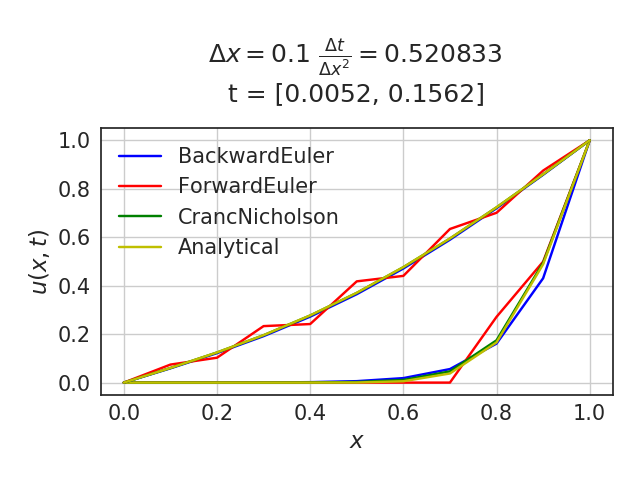
\includegraphics[width=0.99\textwidth]{/home/karl/doc/subj/att/fys4150/project5/resultsKeep/5c/out5CNumber1.png}
		\caption{1D. Coarse mesh. Stability requirement Forward Euler not satisfied.\\ \textit{Forward Euler is unstable, while the other schemes are stable. Backward Euler and Crank-Nicolson produce results close to the anlytical solution for all time steps. Steady state is approached for Backward Euler and Crank-Nicolson.}}
		\label{1}
	\end{figure}
\end{minipage}\hfill
\begin{minipage}{.45\textwidth} 
	\begin{figure}[H]
		\centering
		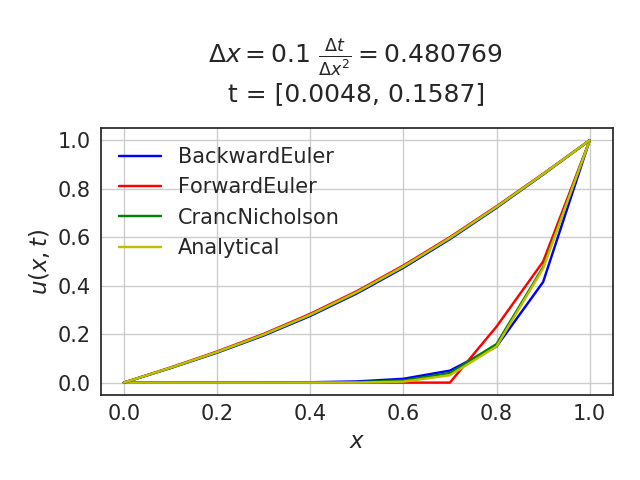
\includegraphics[width=0.99\textwidth]{/home/karl/doc/subj/att/fys4150/project5/resultsKeep/5c/out5CNumber2.png}
		\caption{1D. Coarse mesh. Stability requirement Forward satisfied.\\ \textit{Forward Euler is now stable. All schemes produce results looking qualitively like the analytical solution. Forward Euler has the largest error.}.}
		\label{fig:unzoomed}
	\end{figure}
\end{minipage}\hfill
\vspace{2ex}

From the figures above, we see that the Forward Euler scheme is very sensitive to the stability requriement, implying that a very fine time step is needed for acceptable results for Forward Euler. We also see that the Backward Euler scheme and the Crank-Nicolson scheme are stable regardless of the stability requirement for Forward Euler being satisfied or not. From this point of view, the Backward and Crank-Nicolson schemes are prefered, since they need fewer time steps. All these observations fit well with our numerical findings, that except for Forward Euler, the other schemes are unconditionally stable.\\

The following two figures show the L2-norm for the schemes in the coarse mesh case. The L2-norm is calculated according to

\begin{equation}\label{eq:norm1d}
	|E|_{L^2} = \sqrt{\Delta t \Delta x \sum_{t_j} \sum_{x_j} (u_{Numerical} - u_{Exact})^2},
\end{equation}

so our error-norm contains errors in both space and time.

\begin{minipage}{.45\textwidth} 
	\begin{figure}[H]
		\centering
		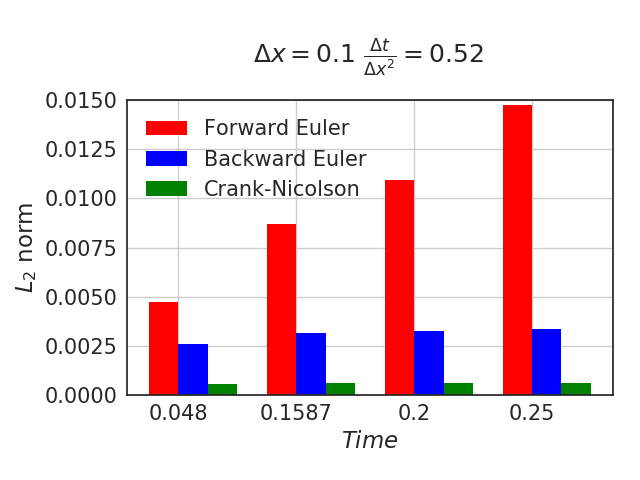
\includegraphics[width=0.99\textwidth]{/home/karl/doc/subj/att/fys4150/project5/resultsKeep/5d/out5NormDx1.png}
		\caption{$L_2$ error norm. 1D. Coarse mesh. Stability requirement Forward Euler not satisfied.\\ \textit{The error-norm increaes with time for Forward Euler when the stability requirement is violated. Crank-Nicolson has the lowest error-norm.}}
		\label{fig:l21}
	\end{figure}
\end{minipage}\hfill
\begin{minipage}{.45\textwidth} 
	\begin{figure}[H]
		\centering
		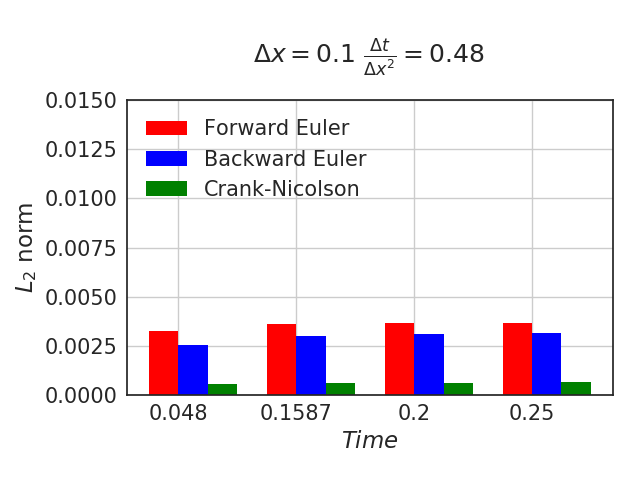
\includegraphics[width=0.99\textwidth]{/home/karl/doc/subj/att/fys4150/project5/resultsKeep/5d/out5NormDx2.png}
		\caption{$L_2$ error norm. 1D. Coarse mesh. Stability requirement Forward satisfied.\\ \textit{When the stability requirement is met, Forward Euler produces error-norms with the same behavior as the other schemes. Crank-Nicolson has the lowest error-norm, while Forward Euler has the highest error-norm. The norms stabilizes as steady state is approached.}}
		\label{fig:l22}
	\end{figure}
\end{minipage}\hfill
\vspace{2ex}

From the above two figures we again see the sensitivity of Forward Euler to its stability requirement. Also we see that Crank-Nicolson is the best scheme, producing the lowest error-norm at all times. \\

To study the schemes error towards equilibrium, we included two more time points in the error-norm figures above. We see that in the stable case, all schemes has error-norms that converges to scheme specific values. This is as expected, since little happends once steady state is reached, adding little to the error-norms.\\ 

The next two figures show the same teo types of discretizations with respect tot he stability requuirement as the figures above, but now the mesh is finer, $\Delta x= 0.01$.

\begin{minipage}{.45\textwidth} 
	\begin{figure}[H]
		\centering
		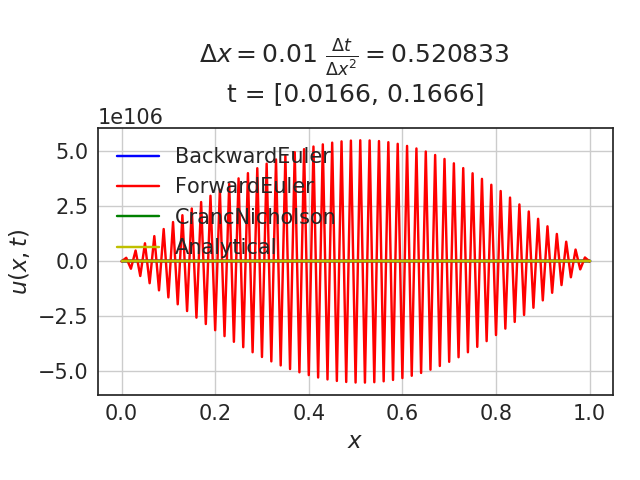
\includegraphics[width=0.99\textwidth]{/home/karl/doc/subj/att/fys4150/project5/resultsKeep/5c/out5CNumber3.png}
		\caption{1D. Fine mesh. Stability requirement Forward Euler not satisfied.\\ \textit{As for the coarse mesh, Forward Euler is unstable.}}
		\label{fig:fig3}
	\end{figure}
\end{minipage}\hfill
\begin{minipage}{.45\textwidth} 
	\begin{figure}[H]
		\centering
		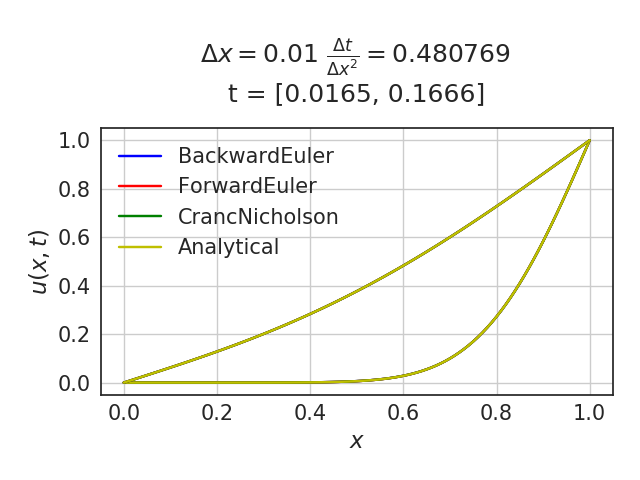
\includegraphics[width=0.99\textwidth]{/home/karl/doc/subj/att/fys4150/project5/resultsKeep/5c/out5CNumber4.png}
		\caption{1D. Fine mesh. Stability requirement Forward satisfied.\\ \textit{Forward Euler is stable. All methods give solutions close to the analytical solution.}}
		\label{fig:1dFineMeshAll}
	\end{figure}
\end{minipage}\hfill
\vspace{2ex}

Again we see the sensitivity of Forward Euler to the stability requirement. A small breach of the stability requirement gives large oscillations, making the solution non-physical. So even if the mesh is much finer compared to the previous figures, this is not enough to avoid unphysical oscillations in the Forward Euler scheme when the stability requirement for Forward Euler is violated. On the other hand, the figure to the right shows that Forward Euler, and the other methods, gives very good fit to the analytical solution when the stability requirement is met.\\

The next figure shows the same as the figure to the left above, with the difference that the results for Froward Euler is removed. Forward Euler is removed so that we can see the solutions of the other two schemes more clearly.

\begin{figure}[H]
	\centering
	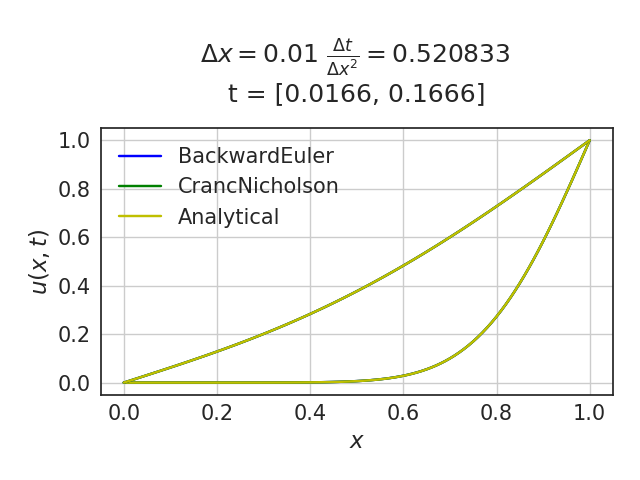
\includegraphics[width=0.6\textwidth]{/home/karl/doc/subj/att/fys4150/project5/resultsKeep/5c/out5CNumber5.png}
	\caption{Same as Figure \ref{fig:fig3} without Forward Euler. \\ \textit{Backward Euler and Crank-Nicolson produces very good results below also when the stability limit for Forward Euler is not satisfied.}}
	\label{1}
\end{figure}

From the figure above we see that both Backward Euler and Crank-Nicolson produces very good results in the case where the stability requirement of Forward Euler is violated.\\

The following two figuers shows the $L_2$-norms for the schemes in the fine mesh case.

\begin{minipage}{.45\textwidth} 
	\begin{figure}[H]
		\centering
		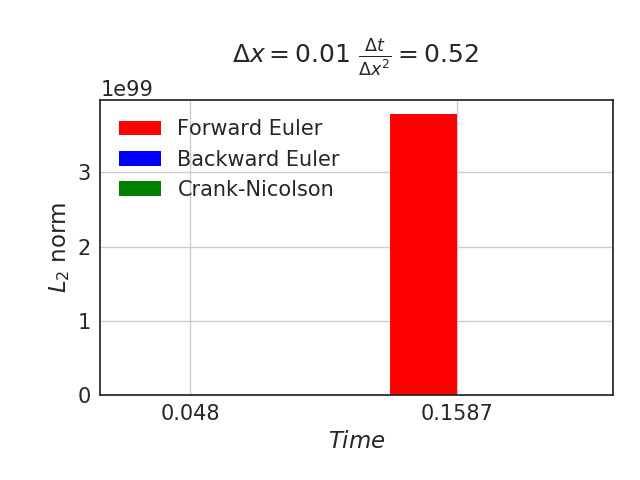
\includegraphics[width=0.99\textwidth]{/home/karl/doc/subj/att/fys4150/project5/resultsKeep/5d/out5NormDx3.png}
		\caption{$L_2$ error norm. 1D. Coarse mesh. Stability requirement Forward Euler not satisfied.\\ \textit{The error-norm for Forward Euler explodes, when the stability requirement is violated.}}
		\label{fig:l23}
	\end{figure}
\end{minipage}\hfill
\begin{minipage}{.45\textwidth} 
	\begin{figure}[H]
		\centering
		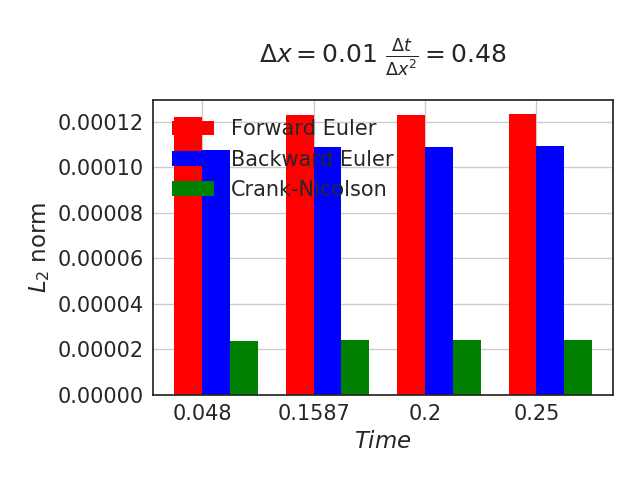
\includegraphics[width=0.99\textwidth]{/home/karl/doc/subj/att/fys4150/project5/resultsKeep/5d/out5NormDx4.png}
		\caption{$L_2$ error norm. 1D. Coarse mesh. Stability requirement Forward satisfied.\\ \textit{The ranking of the three schemes is the same as for the coarse case: Forward Euler is worst, and Crank-Nicolson is best. All errors are smaller compared to the coarse mesh case.}}
		\label{fig:l24}
	\end{figure}
\end{minipage}\hfill
\vspace{2ex}

Figure \ref{fig:l23} confirms the results shown in Figure \ref{fig:fig3}. The wild oscillations in Figure \ref{fig:fig3} gives a large error-norm. Figure \ref{fig:l24} reveals the rankings of the schemes, which was difficult to see from Figure \ref{fig:1dFineMeshAll}. It is pretty clear that the ranking of the schemes when it comes to our error-norm is the same as for the coarse case: Forward Euler being the best and Crank-Nicolson best. We also see that the magnitude of the errors is smaller for all schemes for the fine mesh compared case compared to the coarse mesh case.\\

In order to check that the results from the error-norm figure in the fine mesh case, Figure \ref{fig:l24} correspond with Figure \ref{fig:1dFineMeshAll}, we make a zoom of Figure \ref{fig:1dFineMeshAll}:

\begin{figure}[H]
	\centering
	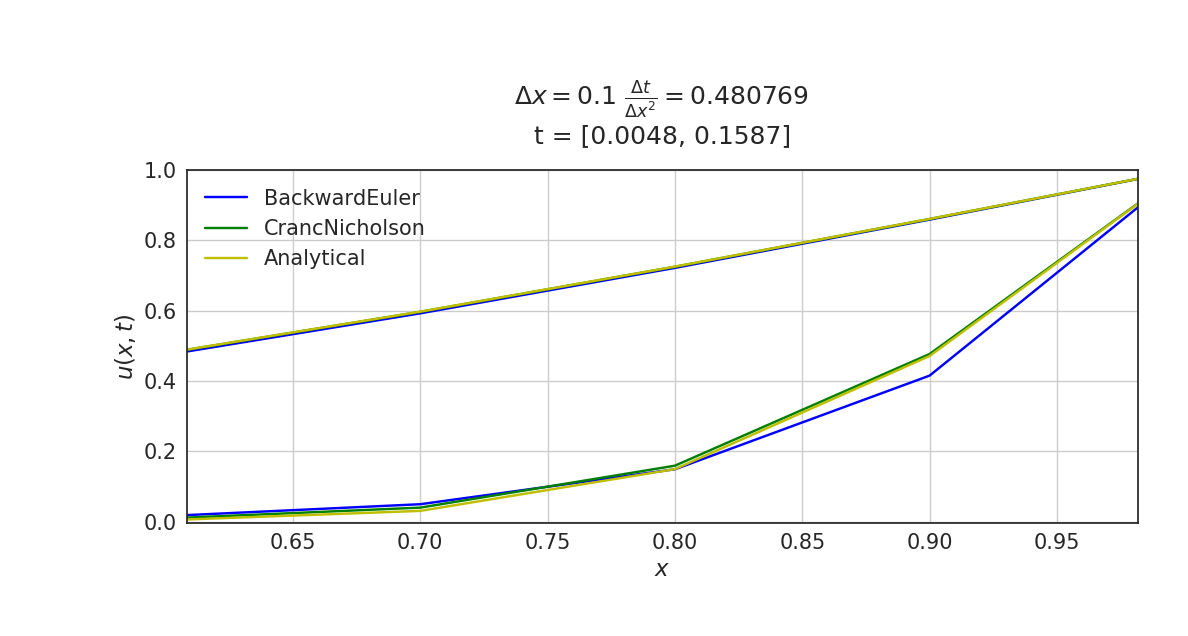
\includegraphics[width=0.6\textwidth]{/home/karl/doc/subj/att/fys4150/project5/resultsKeep/5c/zoomed.png}
	\caption{Same as Figure \ref{fig:unzoomed} without Forward Euler. Zoomed. \\ \textit{Crank-Nicolson is almost identical with analytical solution and outperforms Backward Euler, confirming the results in Figure \ref{fig:l24}.}}
	\label{1}
\end{figure}

From the above figure we see that, compared to the Backward Euler scheme, the Crank-Nicolson scheme is closer to the analytic solution, confirming what was shown in Figure \ref{fig:l24}.\\

The rankings of the schemes are not unexpected, given our derivations in the theory section, where we showed that the Crank-Nicolson scheme is one order higher in time than the other schemes when it comes to truncation error.

\subsection{2D}
The next six figures show the numerical and analytical solutions in the case where the explicit scheme's stability requriement is satisfied. The first row displays the solutions at an early time, while the second row displays the solutions at a later time.
 
\begin{minipage}{.30\textwidth}
	\begin{figure}[H]
		\centering
		\includegraphics[width=0.99\textwidth]{/home/karl/doc/subj/att/fys4150/project5/resultsKeep/5f/safetfy2/tmpAnalytic_0005out5f.png}
		\caption{2D. $\Delta x = 0.1$. $\Delta t = 0.96 \cdot$ stability limit. Early time. Analytical Solution.\\ \textit{}}
		\label{fig:fig2d1}
	\end{figure}
\end{minipage}\hfill
\begin{minipage}{.30\textwidth} 
	\begin{figure}[H]
		\centering
		\includegraphics[width=0.99\textwidth]{/home/karl/doc/subj/att/fys4150/project5/resultsKeep/5f/safetfy2/tmpImplicit_0005out5f.png}
		\caption{2D. $\Delta x = 0.1$. $\Delta t = 0.96 \cdot$ stability limit. Early time. Implicit scheme.\\ \textit{Good fit with analytical solution}}
		\label{fig:fig2d2}
	\end{figure}
\end{minipage}\hfill
\begin{minipage}{.30\textwidth} 
	\begin{figure}[H]
		\centering
		\includegraphics[width=0.99\textwidth]{/home/karl/doc/subj/att/fys4150/project5/resultsKeep/5f/safetfy2/tmpExplicit_0005out5f.png}
		\caption{2D. $\Delta x = 0.1$. $\Delta t = 0.96 \cdot$ stability limit. Early time. Explicit scheme.\\ \textit{Good fit with analytical solution.}}
		\label{fig:fig2d3}
	\end{figure}
\end{minipage}\hfill
\vspace{2ex}

\begin{minipage}{.30\textwidth} 
	\begin{figure}[H]
		\centering
		\includegraphics[width=0.99\textwidth]{/home/karl/doc/subj/att/fys4150/project5/resultsKeep/5f/safetfy2/tmpAnalytic_0021out5f.png}
		\caption{2D. $\Delta x = 0.1$. $\Delta t = 0.96 \cdot$ stability limit. Later time. Analytical Solution.\\ \textit{}}
		\label{fig:fig2d4}
	\end{figure}
\end{minipage}\hfill
\begin{minipage}{.30\textwidth} 
	\begin{figure}[H]
		\centering
		\includegraphics[width=0.99\textwidth]{/home/karl/doc/subj/att/fys4150/project5/resultsKeep/5f/safetfy2/tmpImplicit_0021out5f.png}
		\caption{2D. $\Delta x = 0.1$. $\Delta t = 0.96 \cdot$ stability limit. Later time. Implicit scheme.\\ \textit{Good fit with analytical solution.}}
		\label{fig:fig2d5}
	\end{figure}
\end{minipage}\hfill
\begin{minipage}{.30\textwidth} 
	\begin{figure}[H]
		\centering
		\includegraphics[width=0.99\textwidth]{/home/karl/doc/subj/att/fys4150/project5/resultsKeep/5f/safetfy2/tmpExplicit_0021out5f.png}
		\caption{2D. $\Delta x = 0.1$. $\Delta t = 0.96 \cdot$ stability limit. Later time. Explicit scheme.\\ \textit{Good fit with analytical solution.}}
		\label{fig:fig2d6}
	\end{figure}
\end{minipage}\hfill
\vspace{2ex}

In all figures in this section, the implicit scheme is solved with Jacobi's iteration method.\\

From the figures above, we see that when the stability requirement of the explicit scheme is met, the analytical solution is well approximated by both schemes.\\

The next six figures display the same as the above six figures, but now in the case where the explicit's schemes stability limit is violated. 


\begin{minipage}{.30\textwidth} 
	\begin{figure}[H]
		\centering
		\includegraphics[width=0.99\textwidth]{/home/karl/doc/subj/att/fys4150/project5/resultsKeep/5f/tmpAnalytic_0005out5f.png}
		\caption{2D. $\Delta x = 0.1$. $\Delta t = 1.25 \cdot$ stability limit. Early time. Analytical Solution.\\ \textit{}}
		\label{fig:fig2d7}
	\end{figure}
\end{minipage}\hfill
\begin{minipage}{.30\textwidth} 
	\begin{figure}[H]
		\centering
		\includegraphics[width=0.99\textwidth]{/home/karl/doc/subj/att/fys4150/project5/resultsKeep/5f/tmpImplicit_0005out5f.png}
		\caption{2D. $\Delta x = 0.1$. $\Delta t = 1.25 \cdot$ stability limit. Early time. Implicit scheme.\\ \textit{Implicit scheme still produces results very similar to analytical solution when the stability requirement is satisfied.}}
		\label{fig:fig2d8}
	\end{figure}
\end{minipage}\hfill
\begin{minipage}{.30\textwidth} 
	\begin{figure}[H]
		\centering
		\includegraphics[width=0.99\textwidth]{/home/karl/doc/subj/att/fys4150/project5/resultsKeep/5f/tmpExplicit_0005out5f.png}
		\caption{2D. $\Delta x = 0.1$. $\Delta t = 1.25 \cdot$ stability limit. Early time. Explicit scheme.\\ \textit{Explicit scheme seemingly produces OK results for early times when the stability requirement is violated.}}
		\label{fig:fig2d9}
	\end{figure}
\end{minipage}\hfill
\vspace{2ex}

\begin{minipage}{.30\textwidth} 
	\begin{figure}[H]
		\centering
		\includegraphics[width=0.99\textwidth]{/home/karl/doc/subj/att/fys4150/project5/resultsKeep/5f/tmpAnalytic_0021out5f.png}
		\caption{2D. $\Delta x = 0.1$. $\Delta t = 1.25 \cdot$ stability limit. Later time. Analytical Solution.\\ \textit{}}
		\label{fig:fig2d10}
	\end{figure}
\end{minipage}\hfill
\begin{minipage}{.30\textwidth} 
	\begin{figure}[H]
		\centering
		\includegraphics[width=0.99\textwidth]{/home/karl/doc/subj/att/fys4150/project5/resultsKeep/5f/tmpImplicit_0021out5f.png}
		\caption{2D. $\Delta x = 0.1$. $\Delta t = 1.25 \cdot$ stability limit. Later time. Implicit scheme.\\ \textit{Implicit scheme produces results very similar to analytical solution when the stability requirement is satisfied.}}
		\label{fig:fig2d11}
	\end{figure}
\end{minipage}\hfill
\begin{minipage}{.30\textwidth} 
	\begin{figure}[H]
		\centering
		\includegraphics[width=0.99\textwidth]{/home/karl/doc/subj/att/fys4150/project5/resultsKeep/5f/tmpExplicit_0021out5f.png}
		\caption{2D. $\Delta x = 0.1$. $\Delta t = 1.25 \cdot$ stability limit. Later time. Explicit scheme.\\ \textit{For later time periods the explicit scheme produces unphysical oscilllation when the stability requirement is violated.}}
		\label{fig:fig2d12}
	\end{figure}
\end{minipage}\hfill
\vspace{2ex}

From the above two figures we see once again the sensitivity of the explicit scheme to the stability requirement we derived. We see that a  violation of the stability requirement gives unphysical oscillations in the explicit solution, just as in the 1D case. It seems to take longer time before the instability sets in in the 2D case compared to the 1D case.\\

We note that since the implicit scheme seems to give good fit also when the stability requriement of the explicit scheme is violated, the implicit scheme is less costly computational wise compared to the explicit scheme. With the implicit scheme, for a given space discreatization, a coarser time discretization can be chosen wihout getting bad unphysical results as in the explicit scheme. Once again we observe the good fit with our theoretical derivations that gave that the implicit scheme is unconditinally stable and the explicit scheme being conditionally stable.\\

From the above figure it is hard to judge the performance of the different schemes, and to compare them to each other, especially in the case when the stability requirement is violated. In order to study the perfromance of the schemes closer, we calculate a $L_2$-norm, according to

\begin{equation}\label{eq:ld2d}
	E_{L_2} = \sqrt{\Delta x \Delta y \sum_{x_i} \sum_{y_j} (u_{Numerical} - u_{Analytical})^2}.
\end{equation}

We note that this is not the same kind of norm that we used for the 1D case, (\ref{eq:norm1d}), since we now only calculate the space norm at a given time, so the norm does not include time now.\\

The following two figures show the norm from the figures above.

\begin{minipage}{.45\textwidth} 
	\begin{figure}[H]
		\centering
		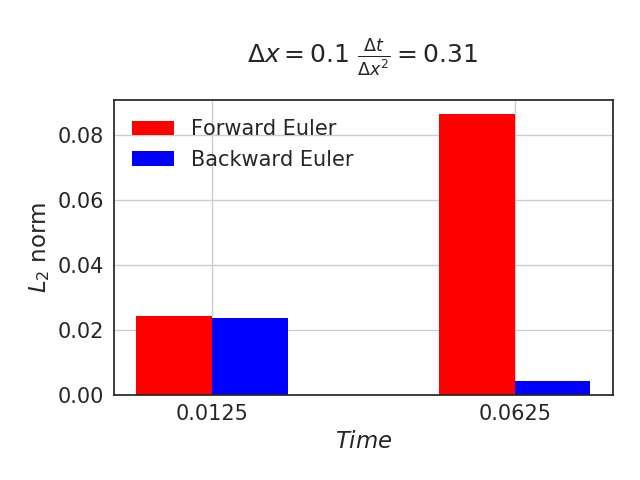
\includegraphics[width=0.99\textwidth]{/home/karl/doc/subj/att/fys4150/project5/resultsKeep/2dnorm/out5Norm2D1.png}
		\caption{$L_2$ error norm. 2D. Coarse mesh. Stability requirement Forward Euler violated.\\ \textit{The error-norm of the explicit schemes explodes when the stability requirement is violated, while the error-norm of the implicit scheme behaves nicely.}}
		\label{fig:norm2d1}
	\end{figure}
\end{minipage}\hfill
\begin{minipage}{.45\textwidth} 
	\begin{figure}[H]
		\centering
		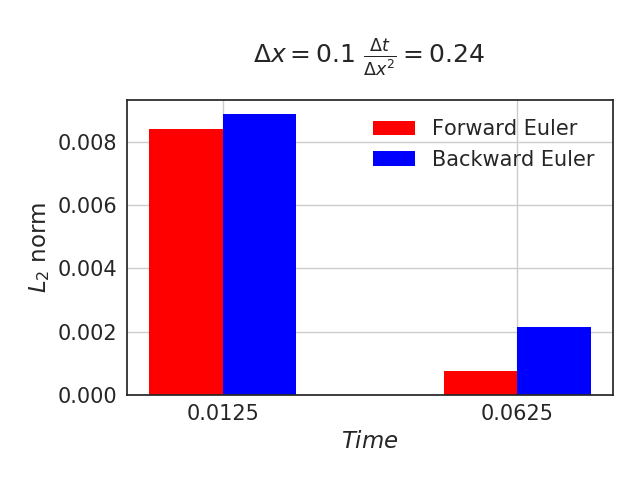
\includegraphics[width=0.99\textwidth]{/home/karl/doc/subj/att/fys4150/project5/resultsKeep/2dnorm/out5Norm2D2.png}
		\caption{$L_2$ error norm. 2D. Coarse mesh. Stability requirement Forward satisfied.\\ \textit{When the stability requirement is met, the explicit scheme is stable and has an error-norm smaller compared to the implicit scheme.}}
		\label{fig:norm2d2}
	\end{figure}
\end{minipage}\hfill
\vspace{2ex}

The left figure above confirms what we already easlily saw from the previous figure, that the explicit schemes error is large when the stability requirement is not satisfied.\\

The right figure shows that also the explicit scheme has stable errors when the stability requriement is satisified. ALso we see that the explicit scheme has a lower error than the omplicit scheme. It is not suprising that the explicit scheme performs better than the implicit scheme whene the stability requirement is satisfied. Firstly, we know from our theoreical derivations that both schemes have the same order of truncation error. Secondly, the fact that the implicit scheme is solved by iterative methods could explain the weaker performance of the implicit scheme. Iterative methods, in contrast to direct methods like the explicit scheme is solved with, are not exact.\\ 

One way to imporve the implicit schemes performance could be by increasing the convergence limit requirements in the iterative scheme. For the simulations behind the convergence limit was $0.00001$. We think it is possible that the implicit scheme could do better with stronger convergence limit. We tested the sensitivity to the convergence requirement, by using a requirement equal to $0.001$, and found that this gave poorer results for the implicit scheme, suggesting that improvements are possible by adjusting the convergence criterion further.

\subsection{Parallelization}
The below two figures show the relation between solution times for the implicit method and the analytical solution. Also the effect of parallization of the analytical solution is shown.

\begin{minipage}{.45\textwidth} 
	\begin{figure}[H]
		\centering
		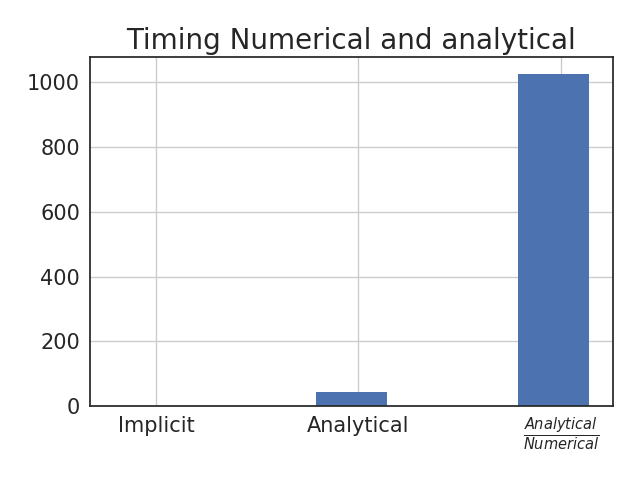
\includegraphics[width=0.99\textwidth]{/home/karl/doc/subj/att/fys4150/project5/resultsKeep/5f/out5fTiming.png}
		\caption{2D. Timing. Numerical scheme: Implicit Jacobi iteration. Analytical solution using 30 points in Gaussian quadrature. \\ \textit{The evaluation of the analytical solution takes 1000 times longer than the numerical solution of the implicit 2D scheme.}}
		\label{fig:figParallel1}
	\end{figure}
\end{minipage}\hfill
\begin{minipage}{.45\textwidth} 
	\begin{figure}[H]
		\centering
		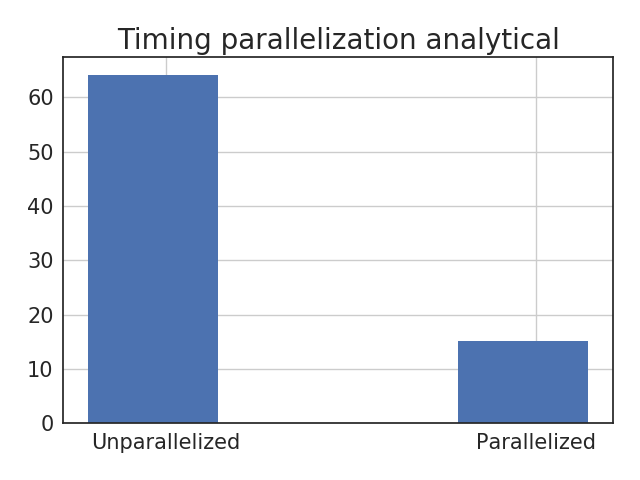
\includegraphics[width=0.99\textwidth]{/home/karl/doc/subj/att/fys4150/project5/resultsKeep/5f/out5gTimingAnalytical.png}
		\caption{2D. Analytical. Times parallelized and unparallelized.\\ \textit{Paralellization of the analytical solution gives a speed by a factor of 4.}}
		\label{fig:figParalell2}
	\end{figure}
\end{minipage}\hfill
\vspace{2ex}

The figure to the left above shows that the evaluation of the analytical solution takes up considerably more time than the solution of the numerical scheme. The reason for this has to do with the analytical function involves a sum of a double integral of a double sum (yes, that is correct), resulting in many loops.\\

We have tried implementing the anaytical solution in an efficient way, by using Gaussian Quadrature with Legendre polynomials. In the lectures we have seen that use of Gaussian quadratue is far less demanding compared to the standard Newton-Cotes integral methods like the trapezoidal and Simpson's rule when it comes to the number of necessary integration points. \\

The huge computational cost of calculating the analytical solution made us parallelize this part of the code (in addition to the implicit Jacobi iteration scheme) using open MP. The figure to the right above shows that the effect of parallizing the analytical solution is a speed up by a factor of 4, which is considerable.

\section{Iterations}
The figure below shows the number of iterations needed for convergence, when applying Jacobi's and Gauss-Seidel's iteration methods to the implicit 2D scheme, for different matrix sizes for the mcoefficient matrix of the linear system.

\begin{minipage}{.45\textwidth} 
	\begin{figure}[H]
		\centering
		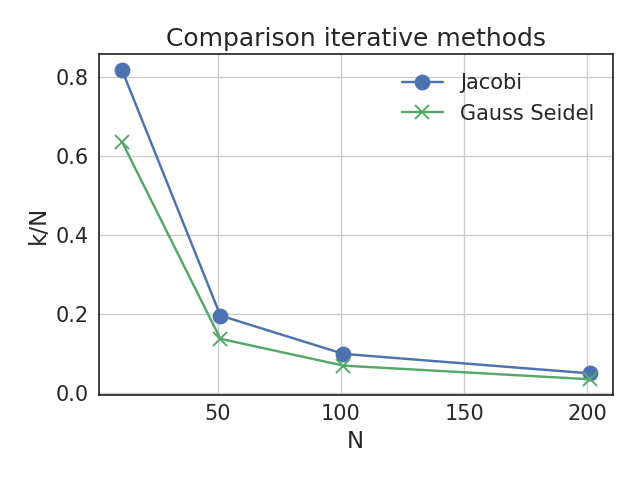
\includegraphics[width=0.99\textwidth]{/home/karl/doc/subj/att/fys4150/project5/resultsKeep/iterations/out5h.png}
		\caption{Number of iterations at the last time step divided by $N$ ($A = N \times N$). Tolerance = $0.001$. \\ \textit{For both schemes the number of iterations considerable lower then $N$, making the iterative methods much faster than the classical direct solvers. Gauss-Seidel needs fewer iterations than Jacobi.}}
		\label{fig:iterations1}
	\end{figure}
\end{minipage}\hfill
\begin{minipage}{.45\textwidth} 
	\begin{figure}[H]
		\centering
		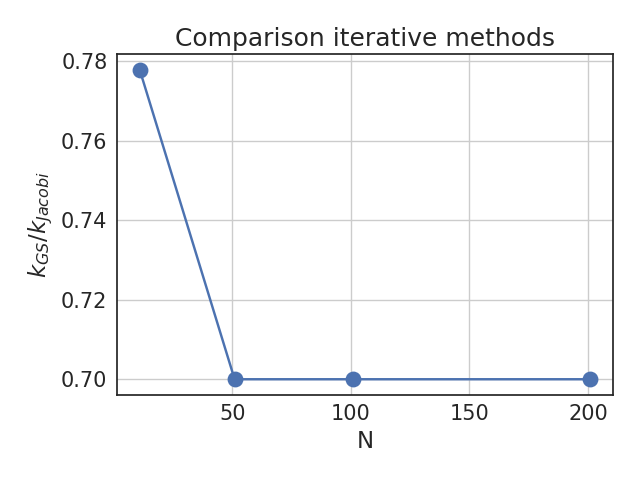
\includegraphics[width=0.99\textwidth]{/home/karl/doc/subj/att/fys4150/project5/resultsKeep/iterations/out5h2.png}
		\caption{Number of iterations in Gauss-Seidel divided by number of iterations Jacobi.\\ \textit{The number of iterations in Gauss-Seidel seems to stabilize to $2/3$ of the number of Jacobi-iterations as the system grows ($N$ increaes), giving a speed up of around $1/3$ going from Jacobi to Gauss-Seidel.}}
		\label{fig:iterations2}
	\end{figure}
\end{minipage}\hfill
\vspace{2ex}

The figure to the left above shows that for both iteration methods the number of iterations reduces to less than 10 per cent of the number of elements in one direction in the coefficient matrix, $N$. From our discussion of FLOP count in the theory section, we know that the fixed point iteration method, which Jacobi and Gauss-Seidel are examples of, is $\mathcal{O}(kN)$ with regards to FLOPS. With the figure above to the left showing that $k < 0.1N$, we get that the iteration methods are considerable more effiecient compared to LU, which goes like $\mathcal{O}(N^2)$ FLOPS, and even faster compared to Gaussian elimination, which goes like $\mathcal{O}(N^3)$ FLOPS, see Hjorth-Jensen \cite{MHJ} p. 173 for FLOP counts on the direct methods.\\

From the figure to the right we see that Gauss-Seidel needs about $2/3$ of the number of iterations that Jacobi needs. This share looks stable as the system increases, that is as $N$ grows.\\ 

The fact that Gauss-Seidel needs $1/3$ less iterations than Jacobi suggests that Gauss-Seidel should be our preffered method for solving the 2D problem with the implicit scheme. However, the Jacobi algorithm is very easy to parallelize, since each point in the loop only depends on previous iterations. From the previous section we have seen that parallelization by Open MP can give a speed up by a factor of 4, which is considerable more than the $1/3$ FLOPS one saves by choosing Gauss-Seidel over Jacobi. Hence by parallizing Jacobi, we get a faster solver compared to running unparallized Gauss-Seidel.\\

The results in the figures above are based on the iteration number for the last time period of simulations. We calcuated the iteration number for all time periods, and the variation in iteration number between time periods was very low, implying that the above figure is representable for all time periods.

\section{Conclusions}
Applying Taylor expansions, we have derived numerical finite difference schemes for both the 1D and the 2D diffusion equation. For the 1D diffusion equation we have derived the Forward Euler scheme, the Backward Euler scheme and the Crank-Nicolson scheme. For the 2D diffusion equation we derived an explicit scheme based on the Forward Euler time derivative approximation, and an implicit scheme, based on the Backward Euler approximation of the time derivative.\\

Truncation errors are derived for all schemes. We find that all schemes have truncation errors that are second order in the space variables, so the truncation error goes like $\mathcal{O}(\Delta h^2)$, where $h$ is a spatial step size. Exepct for the Crank-Nicolson scheme, which is second order also in time, all the other schemes are first order in time.\\

We have performed stability analysis of all schemes, using Neumann stability analysis. Except for the Forward Euler scheme, all schmes are unconditionally stable. The Forward Euler scheme is found to be stable for $\Delta t/\Delta x^2 < 1/2$, in the 1D case, and stable for $\Delta t /h^2 < 1/4$ in the quadratic ($h = \Delta x = \Delta y$) 2D case.\\

Analytical solutions for the 1D and the 2D diffusion equation are derived using the separation of variables technique. \\

The 1D cases are implemented in c++ by using one single scheme, the $\theta$-scheme. We show how all the schemes in the 1D case are special cases of the $\theta$-scheme.\\

Linear system formulations are derived for all schemes. In the 1D case, using the $\theta$-scheme, we find that all the schemes corresponds to versions of a tridiagonal linear systems. For tridiagonal systems, the Thomas algorithm, which is much more efficient with regard to FLOPS compared to Gaussian elimination and LU-decomposition, can, and is, used. We utilize the fact that the coefficients in the coefficient matrix are constants by creating a version of the Thomas algorithm that is more efficient than the original Thomas algorithm. \\

In the 2D case, the linear system is still sparse, but it is no longer tridiagonal. The exlicit scheme is still straight forward to implement, while the implicit scheme no longer can be solved by the Thomas algorithm. Other methods are necessary for obtaining efficient solutions of the implicit 2D scheme.\\ 

Iterative method are potentially very efficient methods solving the kind of system we have in the 2D implicit scheme. We present a general iterative scheme, the fixed point iteration scheme. Conditions for convergence of the iterative systems to the true solutions are presented. We derive a FLOP count of the iterative scheme, and find that it goes like $\mathcal{O}(k N)$ FLOPS, where $k$ is the number of iterations and $N$ is the dimension of the matrix $A$ of the linear system. \\

We present two versions of the general fixed point iteration scheme: the Jacobi method and the Gauss-Seidel method. It is shown how methods relates to the iterative fixed point scheme. We derive and implement algorithms for the 2D implicit scheme for both methods. The number of iterations needed for convergence of the iterative schemes reveals huge savings regards to FLOPS compared to direct methods like Gaussian elimination and LU-decomposition. Gauss-Seidel is shown to be more efficient than Jacbobi, Gauss-Seidel needing only $2/3$ of the iterations of Jacobi.\\

In order to speed up the calculations further, we use parallel computing by applying Open MP. Open MP is applied to the Jacobi solver for the 2D implicit scheme and for the numerical evaluation of the analytical solution. We find that Open MP gives a speed up of these parts of the code by a factor of four.\\

We find that the numerical evaluation of the anlytical solution in 2D takes up considerable more time than evaluation of the numerical schemes! The numerical implementation involves mixes of double sums and double integrals, resulting in many FLOPS. In order to increase the efficiency of the numerical evaluation of the analytical solution, we apply Gaussian quadrature with Legendre polynomials, which is known to be much more efficient compared to standard integral methods like e.g. Simpson's rule, for evaluation of the integral. \\

Our numerical results confirms the theoretical derivations. Forward Euler is sensitive around the stability limit, both in the 1D case and in the 2D case. A slight increase of the time step parameter above the stability limit gives unstable solutions, while a slight decrease of the time step parameter below the stability limit gives stable solutions.\\

For 1D the Backward Euler and Crank-Nicolson seems to perform better compared to the Forward Euler scheme, also when the stability condition for the Forward Euler scheme is satisfied. The Crank-Nicolson scheme looks more precise, giving results closer to the analytical solution, compared to the Backward Euler scheme. This last point was not unexpected, knowing from the theoretical derivations that the truncation error of the Crank-Nicolson scheme is one order higher in time compared to the Backward Euler scheme.\\

Potential extensions to this analysis could be a more detailed analysis of the Gaussian qadrature, comparing it with other integration methods with regards to number of needed points. Introduction of relaxation parameters to the iterative scheme and studying the effect of this on the efficiency is another potential direction of future work.



\begin{thebibliography}{9}
	\bibitem{MHJ} 
	Hjorth-Jensen, M.(2015)
	Computational physics. Lectures fall 2015. 
	\url{https://github.com/CompPhysics/ComputationalPhysics/tree/master/doc/Lectures}
	
	\bibitem{MHJ2}
	\url{https://github.com/CompPhysics/ComputationalPhysics/tree/master/doc/pub/pde}
	
	\bibitem{olver} 
	Olver, P.J and Shakiban, C.(2006)
	Applied linear algebra. Pearson Prentice Hall. 

\end{thebibliography}



\end{document}
